% Repository:  https://github.com/chiehrosswang/TRB_LaTeX_tex
%
% Transportation Research Board conference paper template
% version 4.0 Lite (updates made to be compatible in Overleaf and ShareLaTeX)
%
%
% When numbered option is activated, lines are numbered.
\documentclass[numbered]{trbunofficial}
\usepackage{graphicx}
\usepackage{booktabs}

\newread\somefile
\usepackage{xparse}
\usepackage{natbib}
\bibliographystyle{unsrtnat}
\setcitestyle{round}
% \usepackage[colorlinks=true,linkcolor=blue,citecolor=blue]{hyperref}
% For TRB version hide links
\usepackage[hidelinks]{hyperref}

% Put here what will go to headers as author
\AuthorHeaders{Multimodal spatial availability - the case of low
emission zones in Madrid}
\title{Multimodal spatial availability - the case of low emission zones
in Madrid}

% TODO: add macros for easier formatting of \author.
\author{%
    \textbf{Anastasia Soukhov}\\\textit{Corresponding Author}\\
  PhD Candidate\\
  Department of Earth, Environment and Society, McMaster University,
Canada\\
  \href{mailto:soukhoa@mcmaster.ca}{\nolinkurl{soukhoa@mcmaster.ca}}\\
  \hfill\break
    \textbf{Javier Tarriño Ortiz}\\
  PhD Graduate\\
  Universidad Politécnica de Madrid, Spain\\
  \href{mailto:bob@example.com}{\nolinkurl{bob@example.com}}\\
  \hfill\break
    \textbf{Julio A. Soria-Lara}\\
  Associate Professor\\
  Urban and Regional Planning, Universidad Politécnica de Madrid,
Spain\\
  \href{mailto:derek@example.com}{\nolinkurl{derek@example.com}}\\
  \hfill\break
    \textbf{Antonio Páez}\\
  Associate Professor\\
  Department of Earth, Environment and Society, McMaster University,
Canada\\
  \href{mailto:paezha@mcmaster.ca}{\nolinkurl{paezha@mcmaster.ca}}\\
  \hfill\break
  }

% If necessary modify the number of words per table or figure default is set to
% 250 words per table (default defined in cls)


% If words are counted manually, put that number here. This does not include
% figures and tables. This can also be used to avoid problems with texcount
% program i.e. if one does not have it installed.
\TotalWords{7500}


% tightlist command for lists without linebreak
\providecommand{\tightlist}{%
  \setlength{\itemsep}{0pt}\setlength{\parskip}{0pt}}



\usepackage{multirow}
\usepackage{multicol}
\usepackage{colortbl}
\usepackage{hhline}
\newlength\Oldarrayrulewidth
\newlength\Oldtabcolsep
\usepackage{longtable}
\usepackage{array}
\usepackage{hyperref}
\usepackage{float}
\usepackage{wrapfig}

\begin{document}
\maketitle


\section{Abstract}
An increasing number of studies within the domain of transportation
planning are concerned with the inequities in accessibility to
opportunities. A dimension of these inequities arises from differences
in access by mode type (e.g., commuting using a car as opposed to
transit). However, methods implemented in current accessibility
literature are lacking within the context of multi-modal analysis. This
paper presents an extension of spatial availability, a
singly-constrained competitive accessibility measure, for the context of
multi-modal accessibility analysis. We first illustrate the features of
spatial availability that lend itself to multi-modal analysis. We then
demonstrate its use on the case study of Low Emission Zones in Madrid
(Spain) and highlight how this policy intervention changes the
accessibility of populations using different modes. In summary, spatial
availability can be used to create and interpret multi-modal policy
intervention scenarios unlike previous methods: this creation and
interpretation can help regions envision a more sustainable and
equitable access-to-opportunity landscape.
\hfill\break%
\hfill\break%
\noindent\textit{Keywords}:  Multimodal, Accessibility, Equity, Policy
scenarios, Low emission zones,  
\newpage

\global\setlength{\Oldarrayrulewidth}{\arrayrulewidth}

\global\setlength{\Oldtabcolsep}{\tabcolsep}

\setlength{\tabcolsep}{0pt}

\renewcommand*{\arraystretch}{1.5}



\providecommand{\ascline}[3]{\noalign{\global\arrayrulewidth #1}\arrayrulecolor[HTML]{#2}\cline{#3}}

\begin{longtable}[c]{|p{0.88in}|p{0.41in}|p{1.05in}|p{0.58in}|p{1.05in}|p{0.58in}|p{1.05in}}



\ascline{1.5pt}{666666}{1-7}

\multicolumn{1}{>{\raggedright}m{\dimexpr 0.88in+0\tabcolsep}}{\textcolor[HTML]{000000}{\fontsize{11}{11}\selectfont{i}}} & \multicolumn{1}{>{\raggedright}m{\dimexpr 0.41in+0\tabcolsep}}{\textcolor[HTML]{000000}{\fontsize{11}{11}\selectfont{m}}} & \multicolumn{1}{!{\color[HTML]{666666}\vrule width 1pt}>{\raggedleft}m{\dimexpr 1.05in+0\tabcolsep}}{\textcolor[HTML]{000000}{\fontsize{11}{11}\selectfont{S}}\textcolor[HTML]{000000}{\textsubscript{\fontsize{11}{11}\selectfont{i}}}\textcolor[HTML]{000000}{\textsuperscript{\fontsize{11}{11}\selectfont{m}}}} & \multicolumn{1}{>{\raggedleft}m{\dimexpr 0.58in+0\tabcolsep}}{\textcolor[HTML]{000000}{\fontsize{11}{11}\selectfont{a}}\textcolor[HTML]{000000}{\textsubscript{\fontsize{11}{11}\selectfont{i}}}\textcolor[HTML]{000000}{\textsuperscript{\fontsize{11}{11}\selectfont{m}}}} & \multicolumn{1}{>{\raggedleft}m{\dimexpr 1.05in+0\tabcolsep}}{\textcolor[HTML]{000000}{\fontsize{11}{11}\selectfont{V}}\textcolor[HTML]{000000}{\textsubscript{\fontsize{11}{11}\selectfont{i}}}\textcolor[HTML]{000000}{\textsuperscript{\fontsize{11}{11}\selectfont{m}}}} & \multicolumn{1}{!{\color[HTML]{666666}\vrule width 1pt}>{\raggedleft}m{\dimexpr 0.58in+0\tabcolsep}}{\textcolor[HTML]{000000}{\fontsize{11}{11}\selectfont{a}}\textcolor[HTML]{000000}{\textsubscript{\fontsize{11}{11}\selectfont{i}}}} & \multicolumn{1}{>{\raggedleft}m{\dimexpr 1.05in+0\tabcolsep}}{\textcolor[HTML]{000000}{\fontsize{11}{11}\selectfont{V}}\textcolor[HTML]{000000}{\textsubscript{\fontsize{11}{11}\selectfont{i}}}} \\

\ascline{1.5pt}{666666}{1-7}\endfirsthead 

\ascline{1.5pt}{666666}{1-7}

\multicolumn{1}{>{\raggedright}m{\dimexpr 0.88in+0\tabcolsep}}{\textcolor[HTML]{000000}{\fontsize{11}{11}\selectfont{i}}} & \multicolumn{1}{>{\raggedright}m{\dimexpr 0.41in+0\tabcolsep}}{\textcolor[HTML]{000000}{\fontsize{11}{11}\selectfont{m}}} & \multicolumn{1}{!{\color[HTML]{666666}\vrule width 1pt}>{\raggedleft}m{\dimexpr 1.05in+0\tabcolsep}}{\textcolor[HTML]{000000}{\fontsize{11}{11}\selectfont{S}}\textcolor[HTML]{000000}{\textsubscript{\fontsize{11}{11}\selectfont{i}}}\textcolor[HTML]{000000}{\textsuperscript{\fontsize{11}{11}\selectfont{m}}}} & \multicolumn{1}{>{\raggedleft}m{\dimexpr 0.58in+0\tabcolsep}}{\textcolor[HTML]{000000}{\fontsize{11}{11}\selectfont{a}}\textcolor[HTML]{000000}{\textsubscript{\fontsize{11}{11}\selectfont{i}}}\textcolor[HTML]{000000}{\textsuperscript{\fontsize{11}{11}\selectfont{m}}}} & \multicolumn{1}{>{\raggedleft}m{\dimexpr 1.05in+0\tabcolsep}}{\textcolor[HTML]{000000}{\fontsize{11}{11}\selectfont{V}}\textcolor[HTML]{000000}{\textsubscript{\fontsize{11}{11}\selectfont{i}}}\textcolor[HTML]{000000}{\textsuperscript{\fontsize{11}{11}\selectfont{m}}}} & \multicolumn{1}{!{\color[HTML]{666666}\vrule width 1pt}>{\raggedleft}m{\dimexpr 0.58in+0\tabcolsep}}{\textcolor[HTML]{000000}{\fontsize{11}{11}\selectfont{a}}\textcolor[HTML]{000000}{\textsubscript{\fontsize{11}{11}\selectfont{i}}}} & \multicolumn{1}{>{\raggedleft}m{\dimexpr 1.05in+0\tabcolsep}}{\textcolor[HTML]{000000}{\fontsize{11}{11}\selectfont{V}}\textcolor[HTML]{000000}{\textsubscript{\fontsize{11}{11}\selectfont{i}}}} \\

\ascline{1.5pt}{666666}{1-7}\endhead



\multicolumn{1}{>{\raggedright}m{\dimexpr 0.88in+0\tabcolsep}}{} & \multicolumn{1}{>{\raggedright}m{\dimexpr 0.41in+0\tabcolsep}}{\textcolor[HTML]{000000}{\fontsize{11}{11}\selectfont{x}}} & \multicolumn{1}{!{\color[HTML]{666666}\vrule width 1pt}>{\raggedleft}m{\dimexpr 1.05in+0\tabcolsep}}{\textcolor[HTML]{000000}{\fontsize{11}{11}\selectfont{27,292.18}}} & \multicolumn{1}{>{\raggedleft}m{\dimexpr 0.58in+0\tabcolsep}}{\textcolor[HTML]{000000}{\fontsize{11}{11}\selectfont{0.95}}} & \multicolumn{1}{>{\raggedleft}m{\dimexpr 1.05in+0\tabcolsep}}{\textcolor[HTML]{000000}{\fontsize{11}{11}\selectfont{18,959.86}}} & \multicolumn{1}{!{\color[HTML]{666666}\vrule width 1pt}>{\raggedleft}m{\dimexpr 0.58in+0\tabcolsep}}{} & \multicolumn{1}{>{\raggedleft}m{\dimexpr 1.05in+0\tabcolsep}}{} \\





\multicolumn{1}{>{\raggedright}m{\dimexpr 0.88in+0\tabcolsep}}{\multirow[c]{-2}{*}{\parbox{0.88in}{\raggedright \textcolor[HTML]{000000}{\fontsize{11}{11}\selectfont{A}}}}} & \multicolumn{1}{>{\raggedright}m{\dimexpr 0.41in+0\tabcolsep}}{\textcolor[HTML]{000000}{\fontsize{11}{11}\selectfont{z}}} & \multicolumn{1}{!{\color[HTML]{666666}\vrule width 1pt}>{\raggedleft}m{\dimexpr 1.05in+0\tabcolsep}}{\textcolor[HTML]{000000}{\fontsize{11}{11}\selectfont{44,999.80}}} & \multicolumn{1}{>{\raggedleft}m{\dimexpr 0.58in+0\tabcolsep}}{\textcolor[HTML]{000000}{\fontsize{11}{11}\selectfont{1.56}}} & \multicolumn{1}{>{\raggedleft}m{\dimexpr 1.05in+0\tabcolsep}}{\textcolor[HTML]{000000}{\fontsize{11}{11}\selectfont{46,913.04}}} & \multicolumn{1}{!{\color[HTML]{666666}\vrule width 1pt}>{\raggedleft}m{\dimexpr 0.58in+0\tabcolsep}}{\multirow[c]{-2}{*}{\parbox{0.58in}{\raggedleft \textcolor[HTML]{000000}{\fontsize{11}{11}\selectfont{1.32}}}}} & \multicolumn{1}{>{\raggedleft}m{\dimexpr 1.05in+0\tabcolsep}}{\multirow[c]{-2}{*}{\parbox{1.05in}{\raggedleft \textcolor[HTML]{000000}{\fontsize{11}{11}\selectfont{65,872.91}}}}} \\

\ascline{1pt}{666666}{1-7}



\multicolumn{1}{>{\raggedright}m{\dimexpr 0.88in+0\tabcolsep}}{} & \multicolumn{1}{>{\raggedright}m{\dimexpr 0.41in+0\tabcolsep}}{\textcolor[HTML]{000000}{\fontsize{11}{11}\selectfont{x}}} & \multicolumn{1}{!{\color[HTML]{666666}\vrule width 1pt}>{\raggedleft}m{\dimexpr 1.05in+0\tabcolsep}}{\textcolor[HTML]{000000}{\fontsize{11}{11}\selectfont{27,292.18}}} & \multicolumn{1}{>{\raggedleft}m{\dimexpr 0.58in+0\tabcolsep}}{\textcolor[HTML]{000000}{\fontsize{11}{11}\selectfont{0.62}}} & \multicolumn{1}{>{\raggedleft}m{\dimexpr 1.05in+0\tabcolsep}}{\textcolor[HTML]{000000}{\fontsize{11}{11}\selectfont{30,863.43}}} & \multicolumn{1}{!{\color[HTML]{666666}\vrule width 1pt}>{\raggedleft}m{\dimexpr 0.58in+0\tabcolsep}}{} & \multicolumn{1}{>{\raggedleft}m{\dimexpr 1.05in+0\tabcolsep}}{} \\





\multicolumn{1}{>{\raggedright}m{\dimexpr 0.88in+0\tabcolsep}}{\multirow[c]{-2}{*}{\parbox{0.88in}{\raggedright \textcolor[HTML]{000000}{\fontsize{11}{11}\selectfont{B}}}}} & \multicolumn{1}{>{\raggedright}m{\dimexpr 0.41in+0\tabcolsep}}{\textcolor[HTML]{000000}{\fontsize{11}{11}\selectfont{z}}} & \multicolumn{1}{!{\color[HTML]{666666}\vrule width 1pt}>{\raggedleft}m{\dimexpr 1.05in+0\tabcolsep}}{\textcolor[HTML]{000000}{\fontsize{11}{11}\selectfont{44,999.80}}} & \multicolumn{1}{>{\raggedleft}m{\dimexpr 0.58in+0\tabcolsep}}{\textcolor[HTML]{000000}{\fontsize{11}{11}\selectfont{1.03}}} & \multicolumn{1}{>{\raggedleft}m{\dimexpr 1.05in+0\tabcolsep}}{\textcolor[HTML]{000000}{\fontsize{11}{11}\selectfont{103,391.95}}} & \multicolumn{1}{!{\color[HTML]{666666}\vrule width 1pt}>{\raggedleft}m{\dimexpr 0.58in+0\tabcolsep}}{\multirow[c]{-2}{*}{\parbox{0.58in}{\raggedleft \textcolor[HTML]{000000}{\fontsize{11}{11}\selectfont{0.90}}}}} & \multicolumn{1}{>{\raggedleft}m{\dimexpr 1.05in+0\tabcolsep}}{\multirow[c]{-2}{*}{\parbox{1.05in}{\raggedleft \textcolor[HTML]{000000}{\fontsize{11}{11}\selectfont{134,255.38}}}}} \\

\ascline{1pt}{666666}{1-7}



\multicolumn{1}{>{\raggedright}m{\dimexpr 0.88in+0\tabcolsep}}{} & \multicolumn{1}{>{\raggedright}m{\dimexpr 0.41in+0\tabcolsep}}{\textcolor[HTML]{000000}{\fontsize{11}{11}\selectfont{x}}} & \multicolumn{1}{!{\color[HTML]{666666}\vrule width 1pt}>{\raggedleft}m{\dimexpr 1.05in+0\tabcolsep}}{\textcolor[HTML]{000000}{\fontsize{11}{11}\selectfont{2,240.38}}} & \multicolumn{1}{>{\raggedleft}m{\dimexpr 0.58in+0\tabcolsep}}{\textcolor[HTML]{000000}{\fontsize{11}{11}\selectfont{0.68}}} & \multicolumn{1}{>{\raggedleft}m{\dimexpr 1.05in+0\tabcolsep}}{\textcolor[HTML]{000000}{\fontsize{11}{11}\selectfont{2,034.49}}} & \multicolumn{1}{!{\color[HTML]{666666}\vrule width 1pt}>{\raggedleft}m{\dimexpr 0.58in+0\tabcolsep}}{} & \multicolumn{1}{>{\raggedleft}m{\dimexpr 1.05in+0\tabcolsep}}{} \\





\multicolumn{1}{>{\raggedright}m{\dimexpr 0.88in+0\tabcolsep}}{\multirow[c]{-2}{*}{\parbox{0.88in}{\raggedright \textcolor[HTML]{000000}{\fontsize{11}{11}\selectfont{C}}}}} & \multicolumn{1}{>{\raggedright}m{\dimexpr 0.41in+0\tabcolsep}}{\textcolor[HTML]{000000}{\fontsize{11}{11}\selectfont{z}}} & \multicolumn{1}{!{\color[HTML]{666666}\vrule width 1pt}>{\raggedleft}m{\dimexpr 1.05in+0\tabcolsep}}{\textcolor[HTML]{000000}{\fontsize{11}{11}\selectfont{3,745.89}}} & \multicolumn{1}{>{\raggedleft}m{\dimexpr 0.58in+0\tabcolsep}}{\textcolor[HTML]{000000}{\fontsize{11}{11}\selectfont{1.12}}} & \multicolumn{1}{>{\raggedleft}m{\dimexpr 1.05in+0\tabcolsep}}{\textcolor[HTML]{000000}{\fontsize{11}{11}\selectfont{7,837.22}}} & \multicolumn{1}{!{\color[HTML]{666666}\vrule width 1pt}>{\raggedleft}m{\dimexpr 0.58in+0\tabcolsep}}{\multirow[c]{-2}{*}{\parbox{0.58in}{\raggedleft \textcolor[HTML]{000000}{\fontsize{11}{11}\selectfont{0.99}}}}} & \multicolumn{1}{>{\raggedleft}m{\dimexpr 1.05in+0\tabcolsep}}{\multirow[c]{-2}{*}{\parbox{1.05in}{\raggedleft \textcolor[HTML]{000000}{\fontsize{11}{11}\selectfont{9,871.71}}}}} \\

\ascline{1pt}{666666}{1-7}



\multicolumn{1}{>{\raggedright}m{\dimexpr 0.88in+0\tabcolsep}}{\textcolor[HTML]{000000}{\fontsize{11}{11}\selectfont{TOTALS}}} & \multicolumn{1}{>{\raggedright}m{\dimexpr 0.41in+0\tabcolsep}}{\textcolor[HTML]{000000}{\fontsize{11}{11}\selectfont{}}} & \multicolumn{1}{!{\color[HTML]{666666}\vrule width 1pt}>{\raggedleft}m{\dimexpr 1.05in+0\tabcolsep}}{\textcolor[HTML]{000000}{\fontsize{11}{11}\selectfont{150,570.22}}} & \multicolumn{1}{>{\raggedleft}m{\dimexpr 0.58in+0\tabcolsep}}{\textcolor[HTML]{000000}{\fontsize{11}{11}\selectfont{N/A}}} & \multicolumn{1}{>{\raggedleft}m{\dimexpr 1.05in+0\tabcolsep}}{\textcolor[HTML]{000000}{\fontsize{11}{11}\selectfont{210,000.00}}} & \multicolumn{1}{!{\color[HTML]{666666}\vrule width 1pt}>{\raggedleft}m{\dimexpr 0.58in+0\tabcolsep}}{\textcolor[HTML]{000000}{\fontsize{11}{11}\selectfont{N/A}}} & \multicolumn{1}{>{\raggedleft}m{\dimexpr 1.05in+0\tabcolsep}}{\textcolor[HTML]{000000}{\fontsize{11}{11}\selectfont{210,000.00}}} \\

\ascline{1.5pt}{666666}{1-7}



\end{longtable}



\arrayrulecolor[HTML]{000000}

\global\setlength{\arrayrulewidth}{\Oldarrayrulewidth}

\global\setlength{\tabcolsep}{\Oldtabcolsep}

\renewcommand*{\arraystretch}{1}

\hypertarget{abstract}{%
\section{Abstract}\label{abstract}}

An increasing number of studies within the domain of transport are
concerned with the inequities in accessibility to opportunities. A
dimension of these inequities arise from differences in access by mode
type (e.g., the number of work opportunities that can be reached using a
car as opposed to transit in a city). However, methods assessing
multimodal accessibility in the literature fall short as aspects of
competition for opportunities and the explicit methodological
acknowledgement of opportunities being \emph{finite} are lacking. In
this vein, this paper presents an extension of \emph{spatial
availability}, a singly-constrained competitive accessibility measure,
for the context of multimodal accessibility analysis. We first
illustrate the features of spatial availability that lends itself to
multimodal analysis. We then demonstrate its use on the case study of
Low Emission Zones in Madrid (Spain) and highlight how this policy
intervention changes the accessibility of populations using different
modes. In summary, spatial availability can be used to create and
interpret multimodal policy intervention scenarios unlike previous
methods: this creation and interpretation can help regions envision a
more sustainable and equitable access-to-opportunity landscape by better
identifying differences in accessibility afforded by different modes.

\hypertarget{introduction}{%
\section{Introduction}\label{introduction}}

Implementing urban policies that re-shape cities through accessibility
gains (i.e., the \emph{potential to interact} with opportunities as a
result of land-use mix and transport systems as originally defined by
\citet{hansenHowAccessibilityShapes1959}) have been widely applied
within the transportation literature and is increasingly discussed by
planners
\citep{levinsonTransportAccessManual2020, gowerPlanningInnovationCity2022, siddiqToolsTradeAssessing2021, yanAccessibilityBasedPlanningAddressing2021}.
An important challenge in the identification of interventions that
sustainably and equitably transform cities is the effective evaluation
of \emph{trade-offs}: cities are complex and dynamic ecologies, and
advantaging one component of the city can disadvantage another area,
population, or sub-component In this way, policy evaluation should take
a \emph{systems} approach
\citep{fikselSustainabilityResilienceSystems2006}. One way of
considering systems is from the perspective of the \emph{finite}. As an
illustration, consider the amount of transport space within a city: the
amount is typically finite so re-allocating road space away from one
mode directly impacts the performance of the others (see the literature
on road space reallocation e.g.,
\citet{valencaMainChallengesOpportunities2021}). Evaluating policy
impacts in the context of \emph{finity} provides a way to contextualize
the balance of trade-offs that the citizens of a city should tolerate.

From the perspective of urban transport systems, location-based
accessibility measures have been used in the context of policy
evaluation. For instance, \citet{leeMeasuringImpactsNew2018} assesses
the transit accessibility gains to healthcare and employment
opportunities for disadvantaged neighbourhood in Columbus, Ohio, USA
after the transit system's re-design and introduction of a rapid bus
system. However, a limitation of this study, like others that implement
accessibility measures, is they do not calculate results under a
\emph{constrained} framework i.e., one of \emph{finity}. The citizens of
Columbus should experience qualitative accessibility gains - but is it
at the expense of access to opportunities by other modes? As another
example, \citet{mohriClusteringMethodMeasuring2021} implements a
modified cumulative opportunity measure to assess differences between
private vehicle and transit system accessibility to jobs in Melbourne,
but a similar question remains, does the accessibility afforded to the
private vehicle using population come at the expense of accessibility
losses to transit users?

The two studies discussed in the previous paragraph use
\emph{non-competitive} accessibility measures. There is a branch of
location-based accessibility measures that do incorporate the effect of
competition for opportunities by the population in the region. However,
we argue that these existing methods fall short in acknowledging the
\emph{finity} of opportunities. For instance,
\citet{maoMeasuringSpatialAccessibility2013} applies the competitive
measure, the two-step floating catchment approach (2SFCA) for the case
of access to healthcare services in Florida for both a multimodal
network and a single modal network. While the differences in modal
access are discussed, the question of how the advantage in access
afforded by one mode over another impacts access for different mode
users is unanswered.

This question of how much one mode-using population can access at the
expense of another mode-using population is pertinent equity question in
the evaluation of policy scenarios that are multimodal. For instance,
consider the impact of a low emission zone (LEZ). LEZ is a policy of
spatial and modal discrimination: the circulation of vehicles that are
excessively polluting are restricted in specific areas in a city. In the
recognition that opportunities are finite, the implementation of a LEZ
explicitly reduces the access that the population using polluting
vehicles has to opportunities. This restriction allows the population
using other more sustainable modes to potentially have a higher level of
access than before the LEZ implementation. This evaluation is especially
urgent as LEZ are currently in effect in cities globally; their
reception has been mixed \citep{tarrinoortizPublicAcceptabilityLow2021}
and may be having negative impacts on disadvantaged populations who have
become mobility restricted
\citep{devrijNooneVisitsMe2022, verbeekJustManagementUrban2022}.
Measures that evaluate the accessibility of modes given both
\emph{constrained} and \emph{competitive} considerations are lacking in
the literature, but are needed, to evaluate such policy interventions to
effectively comment on how accessibility changes as a result of the
mobility-restricted mode.

In \citet{soukhovIntroducingSpatialAvailability2023}, we introduce
spatial availability, a type of location-based accessibility measure
that is both \emph{constrained} and \emph{competitive}. In this paper,
we extend the spatial availability measure into a multimodal framework
and explore its use in answering the question outlined: \emph{``given
opportunities are finite, how many are available to a given location
depending on the mode used?''.} The answer to this question quantifies
how many opportunities can be accessed, considering competition, for
different modes. To foreground this exploration, in Section 2, we
discuss short falls of a few existing location-based measures in
comparison to spatial availability through a synthetic example. In
Section 3, the spatial availability of an empirical example of the LEZ
in the city of Madrid, Spain is calculated. We demonstrate how the
restriction of private vehicles with the LEZ implementation impacts the
spatial availability of opportunities for each sub-population using
transit, cycling and walking modes. In Section 4, we provide concluding
remarks on the strengths of the use of spatial availability as a
multi-modal accessibility measure, limitations, and potential future
uses in policy planning scenarios.

\hypertarget{a-brief-review-of-multimodal-accessibility-measurement-methods}{%
\section{A brief review of multimodal accessibility measurement
methods}\label{a-brief-review-of-multimodal-accessibility-measurement-methods}}

Location-based accessibility indicators are quantitative measures of
\emph{potential} interaction with opportunities for locations within a
given region: they are a product of the relationship between land-use
and transport systems. Arguably the most commonly used location-based
measured are cumulative opportunity measures and weighted cumulative
opportunity measures \citep{levinsonTransportAccessManual2020}. These
measures weight the opportunities that can be potentially interacted
with from origin \(i\) to destination \(j\) based on some sort of travel
cost function (e.g., travel time, fare, travel distance) otherwise known
as a travel impedance function \(f^{m}(c^m_{ij})\). Many weighted
cumulative opportunities (often refered to as the gravity-based measure)
originate from the measure proposed by
\citet{hansenHowAccessibilityShapes1959}, which can take the following
multimodal form: \(S_i^m = \sum_j O_j f^m(c_{ij}^m)\) where \(m\) is a
set of modes which have mode-specific travel costs \((c_{ij}^m)\) and
travel impedance functions \(f^m(\cdot)\).

The Hansen-type measure does not consider competition between modes nor
is it constrained. As an example, the work of
\citet{tahmasbiMultimodalAccessibilitybasedEquity2019} uses the
Hansen-type measure to measure the potential interaction with retail
locations using walking, public transit, and car modes \(m\). \(S_i^m\)
is the sum of retail locations \(j\) that can potentially be interacted
with under the travel impedance as calculated for each \(i\) and \(m\).
In other words, each \(i\) has three \(S_i\) values, one per \(m\). In
this work, they demonstrate that the car mode has the highest
\(S_i^{m=car}\) values in the majority of \(i\), i.e., populations using
a car can potentially interact with the most retail opportunities than
populations using other modes. However, the higher \(S_i^{m=car}\)
values are not a result of lower \(S_i^{m}\) values for other modes: it
is not assumed that car-using populations potentially accessing more
opportunities take away potential opportunities for other populations
within the measure. Put another way, this measure does not consider
competition. This measure is also not constrained: there is no global
maximum for \(S_i\) or \(S_i^m\) values, they are presented as a
population normalized accessibility index. This makes the interpretation
of the `potentially interacted opportunities' relative to the region,
making comparisons of the results across different regions challenging.

However, opportunities in a region can be considered finite. There are
only so many school-seats, hospital capacity, food stores, jobs, etc.,
in a region and if one person interacts with an opportunity at a given
time, it is taken. As such, if one person is advantaged and has the
ability to reach more opportunities through a lower travel-cost mode,
than they have more opportunities to potentially interact with more
opportunities than other people. From the other perspective, their are
fewer opportunities left to be potentially interacted with for
populations using higher travel-cost modes. In this way, populations
using modes with a higher travel impedance are at a higher access
disadvantage than populations using lower travel impedance modes. This
recognition is the motivation behind integrating \emph{competition} for
opportunities within multimodal accessibility measures. Arguably one of
the most popular competitive location-based accessibility measures is
the two-step floating catchment area (2SFCA) approach popularized by
\citet{luoMeasuresSpatialAccessibility2003} who simplified the approach
proposed by \citet{shenLocationCharacteristicsInnercity1998} (with
similar considerations for competition in
\citet{weibullAxiomaticApproachMeasurement1976} and
\citet{josephMeasuringPotentialPhysical1982}).

The Shen-type accessibility measure's formulation is:
\(a_i^m = \sum_j \frac{O_jf^m(c_{ij}^m)}{\sum_m D_j^m}\) where \(D_j^m\)
is the potential demand for opportunities equal to travel impedance
weighted population \(\sum_i P_i^m f^m(c_{ij}^m)\). In this way, the
Shen-type measure can be understood as a ratio of the potential
opportunity supply over the potential demand for opportunities. The
measure considers competition, but it is \emph{non-constrained}. A score
of competitive potential accessibility associated is associated with
each location \(i\) for each mode \(m\), but there are no global
maximums. In other words, it is difficult to interpret the meaning of
differences in Shen-type accessibility scores between modes.

To illustrate, \citet{taoInvestigatingImpactsPublic2020a} calculates
\(a_i^m\) to jobs for different income-group populations in Shenzhen
(China) using \(m = \text{public transit}\) and \(m={car}\). They
demonstrate that \(i\)s with low-income populations have lower \(a_i^m\)
than \(i\)s with higher-income populations. Further, they demonstrate
that \(a_i^{m=\text{public transit}}\) is lower than
\(a_i^{m=\text{car}}\) at many \(i\)s, arguing that this may put \(i\)s
with lower-income populations in a further disadvantage. \(a_i\) and/or
\(a_i^m\) are used to compare relative spatial differences in overall
competitive accessibility and modal competitive accessibility, but
because there is no global maximum, making it is difficult to interpret
the significance between differences in \(a_i^{m}\) values. Questions
such as: What is the impact that competition has on the difference in
\(a_i^m\) values? How does impact vary spatially? And what is the
interpretation of this difference? are left unanswered.

Spatial availability improves on previous multi-modal accessibility
approaches as it considers \emph{competition} in the potential
interaction with opportunities in a \emph{constrained} framework (e.g.,
finite opportunities). This is done by considering: 1) competition
between mass effect (e.g., the advantage of sub-populations residing in
relatively low population-density and high opportunity-proximate areas)
and 2) competition between travel impedance (e.g., sub-populations with
relatively low travel-impedance) through a proportional allocation
mechanism. The following sub-section demonstrates how spatial
availability compares to the two other measures and the advantages in
its interpretation through a synthetic example.

\hypertarget{a-synthetic-example-calculating-accessibility-for-multiple-modes-considering-finite-opportunities}{%
\subsection{A synthetic example: calculating accessibility for multiple
modes considering finite
opportunities}\label{a-synthetic-example-calculating-accessibility-for-multiple-modes-considering-finite-opportunities}}

In brief, we define the \emph{spatial availability} at \(i\) ( \(V_{i}\)
) as the proportion of all opportunities in the region \(O\) that are
allocated to location \(i\) from all opportunity destinations \(j\).
\(V_{i}\) is a value of how many opportunities are available to each
location \(i\) out of all the opportunities in the region (e.g., a
neighbourhood has 1,000 spatially available jobs out of 100,000 jobs in
the total region). The general formulation of spatial availability
\(V_{i}\) is shown in Equation (\ref{eq:spatial-availability-general}):

\begin{equation}
\label{eq:spatial-availability-general}
V_i = \sum_{j=1}^J O_jF^t_{ij}
\end{equation}

\noindent where:

\begin{itemize}
\tightlist
\item
  \(F^t_{ij}\) is a balancing factor that depends on the demand for
  opportunities \(O_j\) and cost of movement in the system
  \(f(c_{ij})\).
\item
  \(V_i\) is the number of spatially available opportunities at \(i\);
  the sum of \(V_{i}\) is equivalent to the total sum of opportunities
  in the region (i.e., \(\sum_j O_j = \sum_i V_i\))
\end{itemize}

Spatial availability measure is introduced in
\citet{soukhovIntroducingSpatialAvailability2023}. The unique feature in
the measure is the balancing factor \(F^t_{ij}\), a proportional
allocation mechanisms, which ensures that the \(V_i\) calculated for
each \(i\) sums to the total number of opportunities. Through
\(F^t_{ij}\), spatial availability is a \emph{competitive} and
\emph{constrained} accessibility measure that handles the number of
opportunities in the region in a finite way. \(F^t_{ij}\) consists of
two components: a population-based balancing factor
\(F^p_{i} = \frac{P_i}{\sum_i P_i}\) and an impedance-based balancing
factor \(F^c_{ij} = \frac{F^c_{ij}}{\sum_j F^c_{ij}}\) that,
respectively, allocate opportunities to \(i\) in proportion to the size
of the population at \(i\) (the mass effect) and the cost of reaching
opportunities at \(j\) (the impedance effect). \(F^p_{i}\) and \$
F\^{}c\_\{ij\}\$ are calculated for each \(i\) such that they both equal
1 when summed across all \(i\) in the region (e.g.,
\(\sum_i F^p_{i} = 1\) and \(\sum_i F^c_{ij} = 1\)). These balancing
factors are combined multiplicatively to yield \(F^t_{ij}\) which
ensures that a proportion of the opportunities \(O_j\) are allocated to
each \(i\) accordingly. In other words, assuming a finite number of
opportunities in the region, \(F^t_{ij}\) proportionally allocates
\(O_j\) to each \(i\) such that the resulting \(V_i\) value represents
the number of opportunities \emph{spatially available} to the population
at \(i\). This value can be seen to represent spatial availability as it
is a proportion of the opportunities in the region (i.e.,
\(\sum_j O_j = \sum_i V_i\)).

The focus of this paper is to extend \(V_i\) for multimodal
applications. To do so, the balancing factors are reformulated to yield
a proportional value for the set of modes \(m\) used by populations at
each \(i\). As these factors are proportional, \(F^{pm}_{i}\) and
\(F^{cm}_{ij}\) can be summed up across each \(m\) at each \(i\) and
across all \(i\) to equal to 1. They are also similarly combined
multiplicatively to obtain their joint effect, represented as the
combined balancing factor \(F^{tm}_{ij}\) detailed in Equation
(\ref{eq:multimodal-balancing-factors}).

\begin{equation}
\label{eq:multimodal-balancing-factors}
F^{tm}_{ij} = \frac{F^{pm}_{i} \cdot F^{cm}_{ij}}{\sum_{m=1}^M \sum_{i=1}^N F^{pm}_{i} \cdot F^{cm}_{ij}}
\end{equation}

\noindent Where: - The population balancing factor for each \(m\) at
each \(i\) is \(F^{pm}_{i} = \frac{P_{i}^m}{\sum_{m}\sum_{i} P_{i}^m}\)
- The cost of travel balancing factor for each \(m\) at \(i\) is
\(F_{ij}^{cm} = \frac{f(c_{ij}^m)}{\sum_{m} \sum_{i} f(c_{ij}^m)}\)

Implementing \(F^{tm}_{ij}\), the following Equation
(\ref{eq:spatial-availability-multimodal}) demonstrates the multimodal
configuration of spatial availability \(V_i^m\):

\begin{equation}
\label{eq:spatial-availability-multimodal}
V^m_{i} = \sum_{j=1}^J O_j\ F^{tm}_{ij}
\end{equation}

\noindent Where:

\begin{itemize}
\tightlist
\item
  \(m\) is a set of modes used by populations in the region
  \(m = 1, \cdots, M\).
\item
  \(F^{tm}_{ij}\) is a balancing factor \(F^t_{ij}\) for each \(m\) at
  each \(i\).
\item
  \(V^m_{i}\) is the spatial availability \(V_{i}\) for mode \(m\) at
  each \(i\); the sum of \(V^m_{i}\) for all \(m\) at each \(i\) is
  equivalent to the total sum of opportunities in the region (i.e.,
  \(\sum_j O_j = \sum_i V_i = \sum_{m} \sum_{i} V^m_{i}\))
\end{itemize}

Consider the following synthetic example: Figure \ref{fig:Fig1} depicts
a region with population and jobs at three population centers (\(A\),
\(B\), \(C\)) and three employment centers (\(1\), \(2\), \(3\)). The
population at each population center is divided into two sub-groups, one
using a faster mode \(z\) and another using a slower mode \(x\), to
travel to employment centers. Population center \(A\) is Suburban: it is
closest to its own relatively large employment center at \(A\), close to
the Urban area's equally large employment center \(B\), and has a
population that is smaller than the Urban center \(2\) and larger than
the Satellite center \(3\). The Urban population center has the largest
number of population using slower mode \(x\), followed by the Suburban
then Satellite area. This synthetic example was inspired by the
single-mode example used in
\citet{shenLocationCharacteristicsInnercity1998} and reconfigured in
\citet{soukhovIntroducingSpatialAvailability2023}.

\begin{figure}

{\centering 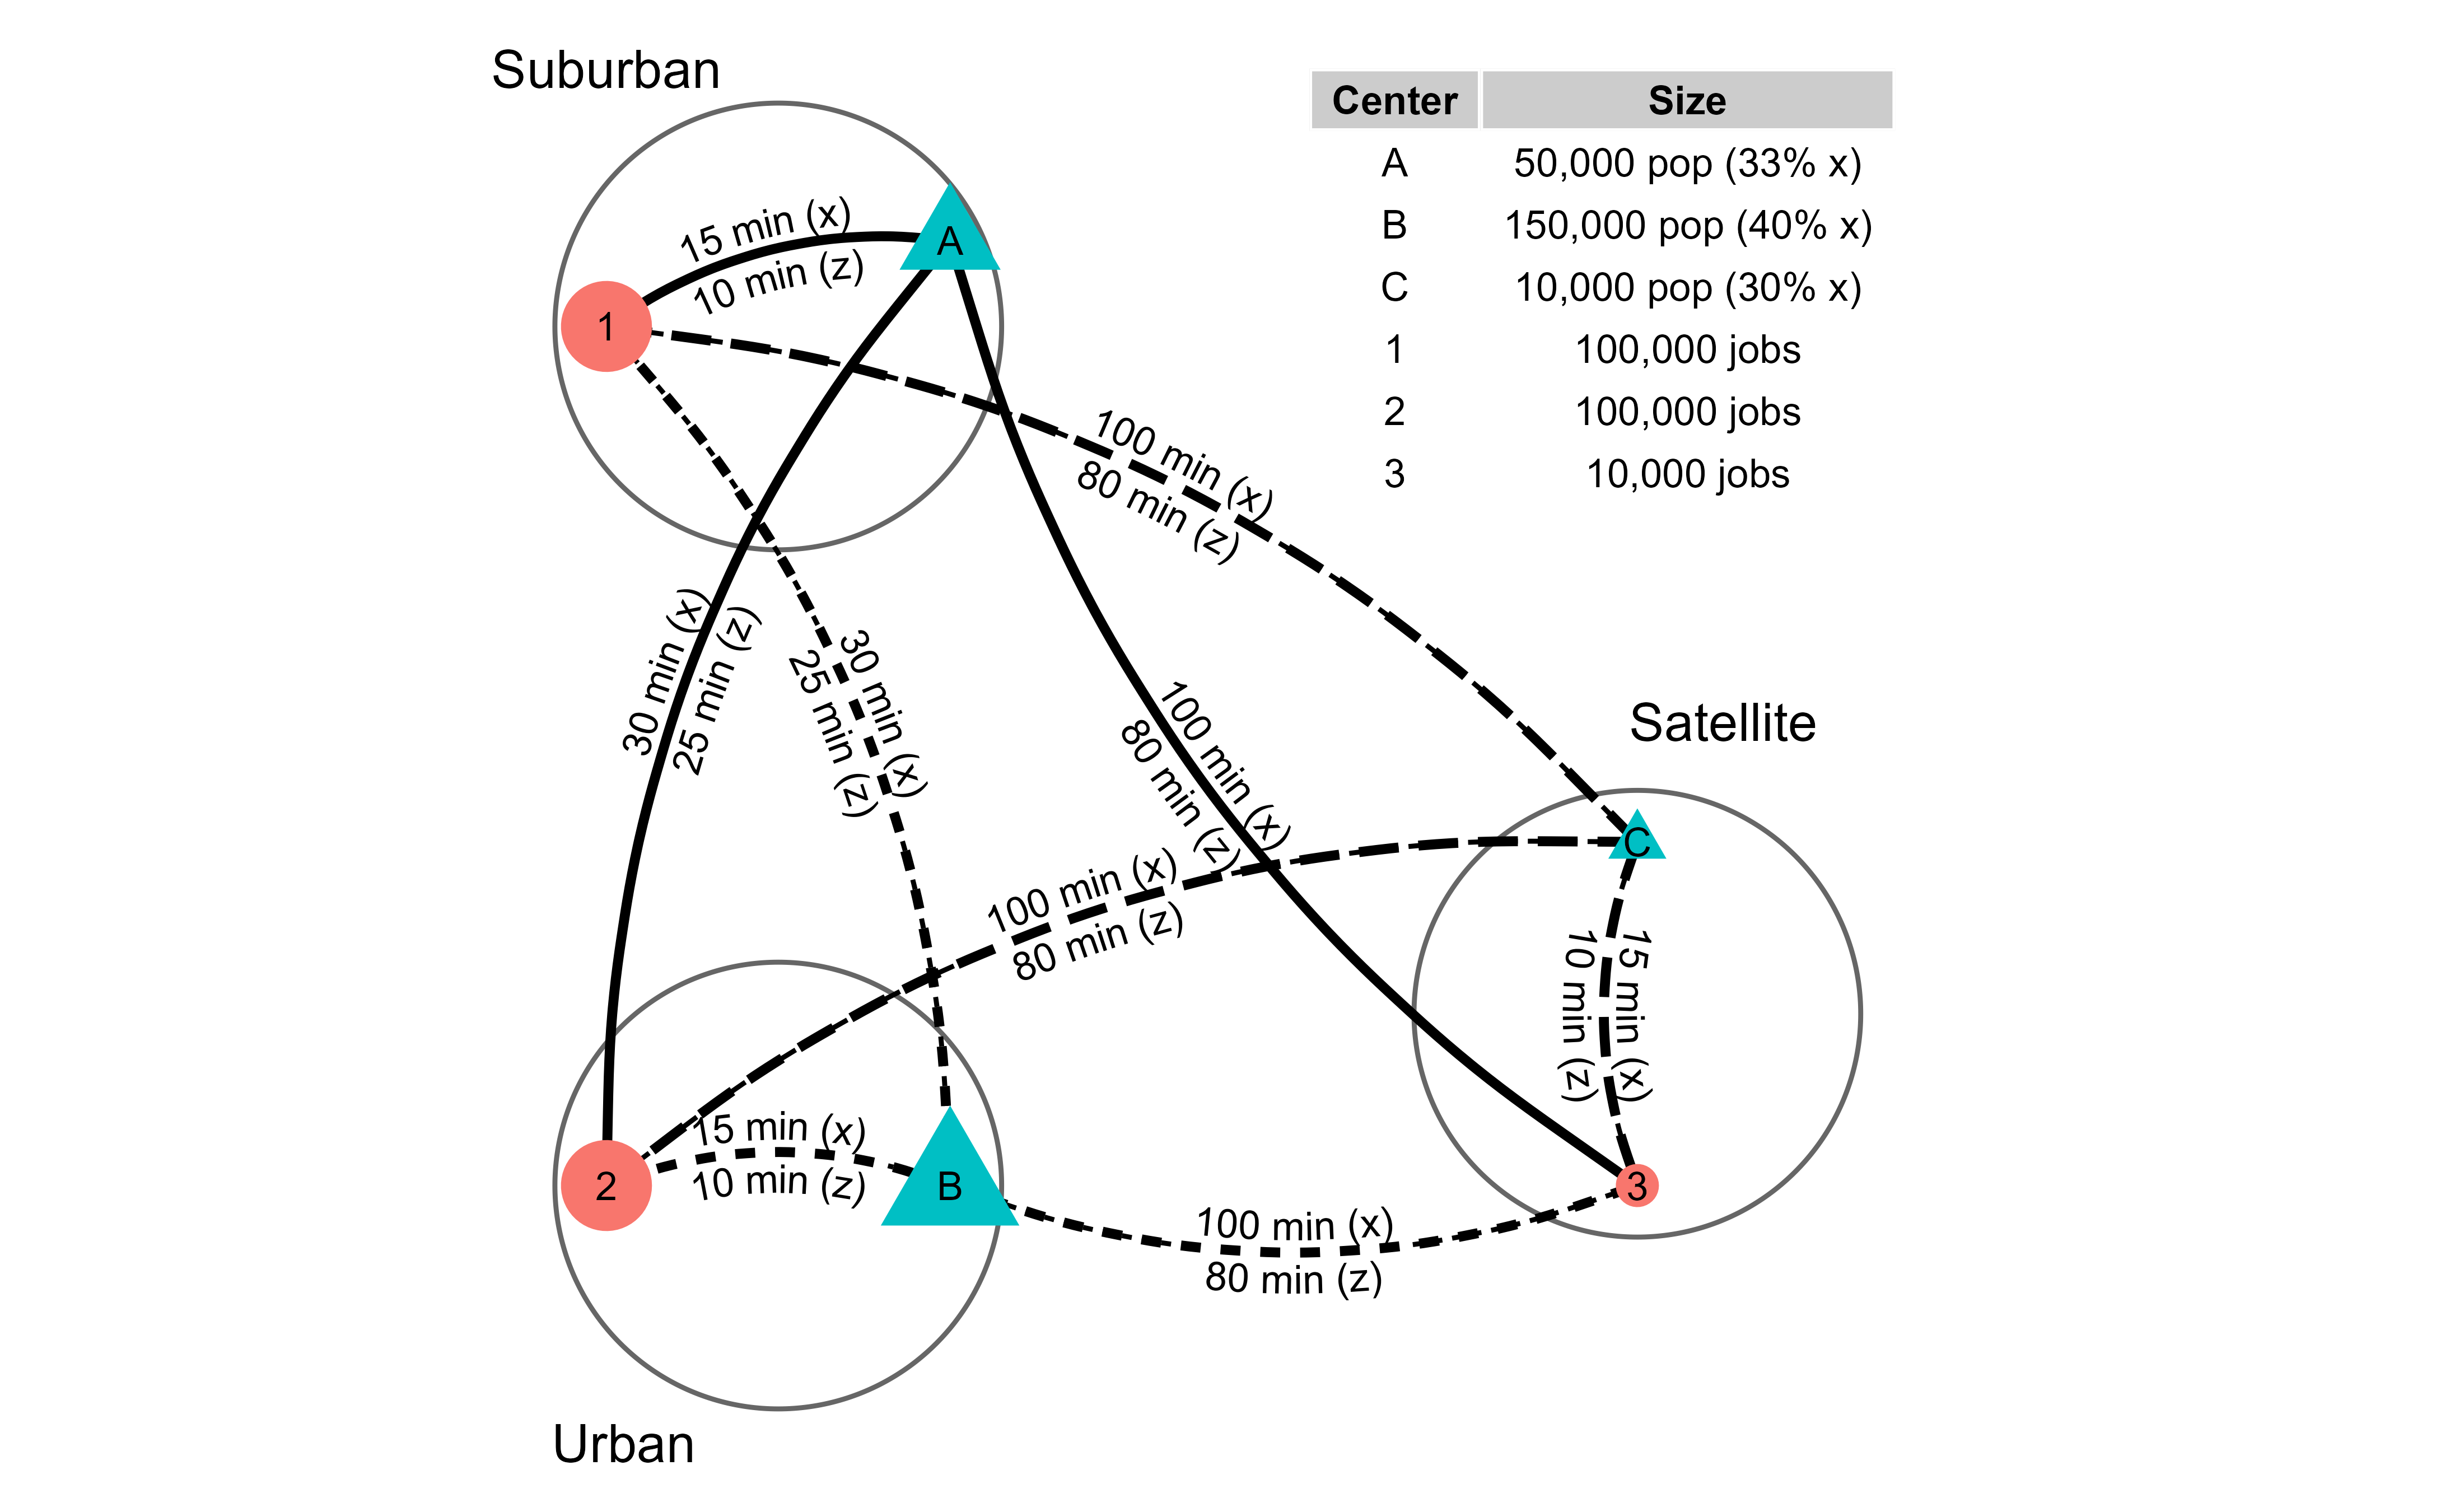
\includegraphics[width=1\linewidth]{images/Fig1} 

}

\caption{\label{fig:Fig1} Modified synthetic example from Shen (1998) with locations of employment centers (in orange), population centers (in blue), number of jobs and population, and travel times for two modes (slower x mode and faster z mode).}\label{fig:synthetic-example-plot}
\end{figure}

From the perspective of access to a \emph{finite} amount of
opportunities in the region (\(210,000\) jobs), the sub-population that
is most proximate to jobs, furthest from densely populated centers, and
is using the lowest travel cost mode \(z\) can potentially access the
most job opportunities. This appears to be the sub-population at
Suburban center \(A\) using the faster mode \(z\). From the other
perspective, sub-populations located further away from jobs, close to
dense populations, and using high cost travel mode \(x\) are at a job
opportunity access \emph{disadvantage} relative to the other
sub-populations. This could be the sub-populations using the slowest
mode \(x\) at either Urban \(B\) or Satellite \(C\) area. From the
perspective of inequities, the competition for opportunities between
different mode-using populations (i.e., how well the land-use and
transport system may serve some and not others), matters.

\global\setlength{\Oldarrayrulewidth}{\arrayrulewidth}

\global\setlength{\Oldtabcolsep}{\tabcolsep}

\setlength{\tabcolsep}{0pt}

\renewcommand*{\arraystretch}{1.5}



\providecommand{\ascline}[3]{\noalign{\global\arrayrulewidth #1}\arrayrulecolor[HTML]{#2}\cline{#3}}

\begin{longtable}[c]{|p{0.88in}|p{0.41in}|p{1.05in}|p{1.05in}|p{0.58in}|p{1.05in}|p{0.58in}}

\caption{Summary\ description\ of\ the\ synthetic\ example:\ accessibility\ values\ at\ each\ origin\ per\ mode\ m\ at\ each\ origin\ i\ and\ aggregated\ between\ modes\ for\ each\ i.}\\

\ascline{1.5pt}{666666}{1-7}

\multicolumn{1}{>{\raggedright}m{\dimexpr 0.88in+0\tabcolsep}}{\textcolor[HTML]{000000}{\fontsize{11}{11}\selectfont{i}}} & \multicolumn{1}{>{\raggedright}m{\dimexpr 0.41in+0\tabcolsep}}{\textcolor[HTML]{000000}{\fontsize{11}{11}\selectfont{m}}} & \multicolumn{1}{!{\color[HTML]{666666}\vrule width 1pt}>{\raggedleft}m{\dimexpr 1.05in+0\tabcolsep}}{\textcolor[HTML]{000000}{\fontsize{11}{11}\selectfont{V}}\textcolor[HTML]{000000}{\textsubscript{\fontsize{11}{11}\selectfont{i}}}\textcolor[HTML]{000000}{\textsuperscript{\fontsize{11}{11}\selectfont{m}}}} & \multicolumn{1}{>{\raggedleft}m{\dimexpr 1.05in+0\tabcolsep}}{\textcolor[HTML]{000000}{\fontsize{11}{11}\selectfont{S}}\textcolor[HTML]{000000}{\textsubscript{\fontsize{11}{11}\selectfont{i}}}\textcolor[HTML]{000000}{\textsuperscript{\fontsize{11}{11}\selectfont{m}}}} & \multicolumn{1}{>{\raggedleft}m{\dimexpr 0.58in+0\tabcolsep}}{\textcolor[HTML]{000000}{\fontsize{11}{11}\selectfont{a}}\textcolor[HTML]{000000}{\textsubscript{\fontsize{11}{11}\selectfont{i}}}\textcolor[HTML]{000000}{\textsuperscript{\fontsize{11}{11}\selectfont{m}}}} & \multicolumn{1}{!{\color[HTML]{666666}\vrule width 1pt}>{\raggedleft}m{\dimexpr 1.05in+0\tabcolsep}}{\textcolor[HTML]{000000}{\fontsize{11}{11}\selectfont{V}}\textcolor[HTML]{000000}{\textsubscript{\fontsize{11}{11}\selectfont{i}}}} & \multicolumn{1}{>{\raggedleft}m{\dimexpr 0.58in+0\tabcolsep}}{\textcolor[HTML]{000000}{\fontsize{11}{11}\selectfont{a}}\textcolor[HTML]{000000}{\textsubscript{\fontsize{11}{11}\selectfont{i}}}} \\

\ascline{1.5pt}{666666}{1-7}\endfirsthead \caption[]{Summary\ description\ of\ the\ synthetic\ example:\ accessibility\ values\ at\ each\ origin\ per\ mode\ m\ at\ each\ origin\ i\ and\ aggregated\ between\ modes\ for\ each\ i.}\\

\ascline{1.5pt}{666666}{1-7}

\multicolumn{1}{>{\raggedright}m{\dimexpr 0.88in+0\tabcolsep}}{\textcolor[HTML]{000000}{\fontsize{11}{11}\selectfont{i}}} & \multicolumn{1}{>{\raggedright}m{\dimexpr 0.41in+0\tabcolsep}}{\textcolor[HTML]{000000}{\fontsize{11}{11}\selectfont{m}}} & \multicolumn{1}{!{\color[HTML]{666666}\vrule width 1pt}>{\raggedleft}m{\dimexpr 1.05in+0\tabcolsep}}{\textcolor[HTML]{000000}{\fontsize{11}{11}\selectfont{V}}\textcolor[HTML]{000000}{\textsubscript{\fontsize{11}{11}\selectfont{i}}}\textcolor[HTML]{000000}{\textsuperscript{\fontsize{11}{11}\selectfont{m}}}} & \multicolumn{1}{>{\raggedleft}m{\dimexpr 1.05in+0\tabcolsep}}{\textcolor[HTML]{000000}{\fontsize{11}{11}\selectfont{S}}\textcolor[HTML]{000000}{\textsubscript{\fontsize{11}{11}\selectfont{i}}}\textcolor[HTML]{000000}{\textsuperscript{\fontsize{11}{11}\selectfont{m}}}} & \multicolumn{1}{>{\raggedleft}m{\dimexpr 0.58in+0\tabcolsep}}{\textcolor[HTML]{000000}{\fontsize{11}{11}\selectfont{a}}\textcolor[HTML]{000000}{\textsubscript{\fontsize{11}{11}\selectfont{i}}}\textcolor[HTML]{000000}{\textsuperscript{\fontsize{11}{11}\selectfont{m}}}} & \multicolumn{1}{!{\color[HTML]{666666}\vrule width 1pt}>{\raggedleft}m{\dimexpr 1.05in+0\tabcolsep}}{\textcolor[HTML]{000000}{\fontsize{11}{11}\selectfont{V}}\textcolor[HTML]{000000}{\textsubscript{\fontsize{11}{11}\selectfont{i}}}} & \multicolumn{1}{>{\raggedleft}m{\dimexpr 0.58in+0\tabcolsep}}{\textcolor[HTML]{000000}{\fontsize{11}{11}\selectfont{a}}\textcolor[HTML]{000000}{\textsubscript{\fontsize{11}{11}\selectfont{i}}}} \\

\ascline{1.5pt}{666666}{1-7}\endhead



\multicolumn{1}{>{\raggedright}m{\dimexpr 0.88in+0\tabcolsep}}{} & \multicolumn{1}{>{\raggedright}m{\dimexpr 0.41in+0\tabcolsep}}{\textcolor[HTML]{000000}{\fontsize{11}{11}\selectfont{x}}} & \multicolumn{1}{!{\color[HTML]{666666}\vrule width 1pt}>{\raggedleft}m{\dimexpr 1.05in+0\tabcolsep}}{\textcolor[HTML]{000000}{\fontsize{11}{11}\selectfont{18,959.86}}} & \multicolumn{1}{>{\raggedleft}m{\dimexpr 1.05in+0\tabcolsep}}{\textcolor[HTML]{000000}{\fontsize{11}{11}\selectfont{27,292.18}}} & \multicolumn{1}{>{\raggedleft}m{\dimexpr 0.58in+0\tabcolsep}}{\textcolor[HTML]{000000}{\fontsize{11}{11}\selectfont{0.95}}} & \multicolumn{1}{!{\color[HTML]{666666}\vrule width 1pt}>{\raggedleft}m{\dimexpr 1.05in+0\tabcolsep}}{\textcolor[HTML]{000000}{\fontsize{11}{11}\selectfont{65,872.91}}} & \multicolumn{1}{>{\raggedleft}m{\dimexpr 0.58in+0\tabcolsep}}{} \\





\multicolumn{1}{>{\raggedright}m{\dimexpr 0.88in+0\tabcolsep}}{\multirow[c]{-2}{*}{\parbox{0.88in}{\raggedright \textcolor[HTML]{000000}{\fontsize{11}{11}\selectfont{A}}}}} & \multicolumn{1}{>{\raggedright}m{\dimexpr 0.41in+0\tabcolsep}}{\textcolor[HTML]{000000}{\fontsize{11}{11}\selectfont{z}}} & \multicolumn{1}{!{\color[HTML]{666666}\vrule width 1pt}>{\raggedleft}m{\dimexpr 1.05in+0\tabcolsep}}{\textcolor[HTML]{000000}{\fontsize{11}{11}\selectfont{46,913.04}}} & \multicolumn{1}{>{\raggedleft}m{\dimexpr 1.05in+0\tabcolsep}}{\textcolor[HTML]{000000}{\fontsize{11}{11}\selectfont{44,999.80}}} & \multicolumn{1}{>{\raggedleft}m{\dimexpr 0.58in+0\tabcolsep}}{\textcolor[HTML]{000000}{\fontsize{11}{11}\selectfont{1.56}}} & \multicolumn{1}{!{\color[HTML]{666666}\vrule width 1pt}>{\raggedleft}m{\dimexpr 1.05in+0\tabcolsep}}{\textcolor[HTML]{000000}{\fontsize{11}{11}\selectfont{65,872.91}}} & \multicolumn{1}{>{\raggedleft}m{\dimexpr 0.58in+0\tabcolsep}}{\multirow[c]{-2}{*}{\parbox{0.58in}{\raggedleft \textcolor[HTML]{000000}{\fontsize{11}{11}\selectfont{1.32}}}}} \\

\ascline{1pt}{666666}{1-7}



\multicolumn{1}{>{\raggedright}m{\dimexpr 0.88in+0\tabcolsep}}{} & \multicolumn{1}{>{\raggedright}m{\dimexpr 0.41in+0\tabcolsep}}{\textcolor[HTML]{000000}{\fontsize{11}{11}\selectfont{x}}} & \multicolumn{1}{!{\color[HTML]{666666}\vrule width 1pt}>{\raggedleft}m{\dimexpr 1.05in+0\tabcolsep}}{\textcolor[HTML]{000000}{\fontsize{11}{11}\selectfont{30,863.43}}} & \multicolumn{1}{>{\raggedleft}m{\dimexpr 1.05in+0\tabcolsep}}{\textcolor[HTML]{000000}{\fontsize{11}{11}\selectfont{27,292.18}}} & \multicolumn{1}{>{\raggedleft}m{\dimexpr 0.58in+0\tabcolsep}}{\textcolor[HTML]{000000}{\fontsize{11}{11}\selectfont{0.62}}} & \multicolumn{1}{!{\color[HTML]{666666}\vrule width 1pt}>{\raggedleft}m{\dimexpr 1.05in+0\tabcolsep}}{\textcolor[HTML]{000000}{\fontsize{11}{11}\selectfont{134,255.38}}} & \multicolumn{1}{>{\raggedleft}m{\dimexpr 0.58in+0\tabcolsep}}{} \\





\multicolumn{1}{>{\raggedright}m{\dimexpr 0.88in+0\tabcolsep}}{\multirow[c]{-2}{*}{\parbox{0.88in}{\raggedright \textcolor[HTML]{000000}{\fontsize{11}{11}\selectfont{B}}}}} & \multicolumn{1}{>{\raggedright}m{\dimexpr 0.41in+0\tabcolsep}}{\textcolor[HTML]{000000}{\fontsize{11}{11}\selectfont{z}}} & \multicolumn{1}{!{\color[HTML]{666666}\vrule width 1pt}>{\raggedleft}m{\dimexpr 1.05in+0\tabcolsep}}{\textcolor[HTML]{000000}{\fontsize{11}{11}\selectfont{103,391.95}}} & \multicolumn{1}{>{\raggedleft}m{\dimexpr 1.05in+0\tabcolsep}}{\textcolor[HTML]{000000}{\fontsize{11}{11}\selectfont{44,999.80}}} & \multicolumn{1}{>{\raggedleft}m{\dimexpr 0.58in+0\tabcolsep}}{\textcolor[HTML]{000000}{\fontsize{11}{11}\selectfont{1.03}}} & \multicolumn{1}{!{\color[HTML]{666666}\vrule width 1pt}>{\raggedleft}m{\dimexpr 1.05in+0\tabcolsep}}{\textcolor[HTML]{000000}{\fontsize{11}{11}\selectfont{134,255.38}}} & \multicolumn{1}{>{\raggedleft}m{\dimexpr 0.58in+0\tabcolsep}}{\multirow[c]{-2}{*}{\parbox{0.58in}{\raggedleft \textcolor[HTML]{000000}{\fontsize{11}{11}\selectfont{0.90}}}}} \\

\ascline{1pt}{666666}{1-7}



\multicolumn{1}{>{\raggedright}m{\dimexpr 0.88in+0\tabcolsep}}{} & \multicolumn{1}{>{\raggedright}m{\dimexpr 0.41in+0\tabcolsep}}{\textcolor[HTML]{000000}{\fontsize{11}{11}\selectfont{x}}} & \multicolumn{1}{!{\color[HTML]{666666}\vrule width 1pt}>{\raggedleft}m{\dimexpr 1.05in+0\tabcolsep}}{\textcolor[HTML]{000000}{\fontsize{11}{11}\selectfont{2,034.49}}} & \multicolumn{1}{>{\raggedleft}m{\dimexpr 1.05in+0\tabcolsep}}{\textcolor[HTML]{000000}{\fontsize{11}{11}\selectfont{2,240.38}}} & \multicolumn{1}{>{\raggedleft}m{\dimexpr 0.58in+0\tabcolsep}}{\textcolor[HTML]{000000}{\fontsize{11}{11}\selectfont{0.68}}} & \multicolumn{1}{!{\color[HTML]{666666}\vrule width 1pt}>{\raggedleft}m{\dimexpr 1.05in+0\tabcolsep}}{\textcolor[HTML]{000000}{\fontsize{11}{11}\selectfont{9,871.71}}} & \multicolumn{1}{>{\raggedleft}m{\dimexpr 0.58in+0\tabcolsep}}{} \\





\multicolumn{1}{>{\raggedright}m{\dimexpr 0.88in+0\tabcolsep}}{\multirow[c]{-2}{*}{\parbox{0.88in}{\raggedright \textcolor[HTML]{000000}{\fontsize{11}{11}\selectfont{C}}}}} & \multicolumn{1}{>{\raggedright}m{\dimexpr 0.41in+0\tabcolsep}}{\textcolor[HTML]{000000}{\fontsize{11}{11}\selectfont{z}}} & \multicolumn{1}{!{\color[HTML]{666666}\vrule width 1pt}>{\raggedleft}m{\dimexpr 1.05in+0\tabcolsep}}{\textcolor[HTML]{000000}{\fontsize{11}{11}\selectfont{7,837.22}}} & \multicolumn{1}{>{\raggedleft}m{\dimexpr 1.05in+0\tabcolsep}}{\textcolor[HTML]{000000}{\fontsize{11}{11}\selectfont{3,745.89}}} & \multicolumn{1}{>{\raggedleft}m{\dimexpr 0.58in+0\tabcolsep}}{\textcolor[HTML]{000000}{\fontsize{11}{11}\selectfont{1.12}}} & \multicolumn{1}{!{\color[HTML]{666666}\vrule width 1pt}>{\raggedleft}m{\dimexpr 1.05in+0\tabcolsep}}{\textcolor[HTML]{000000}{\fontsize{11}{11}\selectfont{9,871.71}}} & \multicolumn{1}{>{\raggedleft}m{\dimexpr 0.58in+0\tabcolsep}}{\multirow[c]{-2}{*}{\parbox{0.58in}{\raggedleft \textcolor[HTML]{000000}{\fontsize{11}{11}\selectfont{0.99}}}}} \\

\ascline{1pt}{666666}{1-7}



\multicolumn{1}{>{\raggedright}m{\dimexpr 0.88in+0\tabcolsep}}{\textcolor[HTML]{000000}{\fontsize{11}{11}\selectfont{TOTALS}}} & \multicolumn{1}{>{\raggedright}m{\dimexpr 0.41in+0\tabcolsep}}{\textcolor[HTML]{000000}{\fontsize{11}{11}\selectfont{}}} & \multicolumn{1}{!{\color[HTML]{666666}\vrule width 1pt}>{\raggedleft}m{\dimexpr 1.05in+0\tabcolsep}}{\textcolor[HTML]{000000}{\fontsize{11}{11}\selectfont{210,000.00}}} & \multicolumn{1}{>{\raggedleft}m{\dimexpr 1.05in+0\tabcolsep}}{\textcolor[HTML]{000000}{\fontsize{11}{11}\selectfont{150,570.22}}} & \multicolumn{1}{>{\raggedleft}m{\dimexpr 0.58in+0\tabcolsep}}{\textcolor[HTML]{000000}{\fontsize{11}{11}\selectfont{N/A}}} & \multicolumn{1}{!{\color[HTML]{666666}\vrule width 1pt}>{\raggedleft}m{\dimexpr 1.05in+0\tabcolsep}}{\textcolor[HTML]{000000}{\fontsize{11}{11}\selectfont{210,000.00}}} & \multicolumn{1}{>{\raggedleft}m{\dimexpr 0.58in+0\tabcolsep}}{\textcolor[HTML]{000000}{\fontsize{11}{11}\selectfont{N/A}}} \\

\ascline{1.5pt}{666666}{1-7}



\end{longtable}



\arrayrulecolor[HTML]{000000}

\global\setlength{\arrayrulewidth}{\Oldarrayrulewidth}

\global\setlength{\tabcolsep}{\Oldtabcolsep}

\renewcommand*{\arraystretch}{1}

The calculated \(S_i^m\), \(a_i^m\) and \(V_i^m\) accessibility values
for each \(i\) and \(m\) are shown in the middle three columns and are
aggregated for each \(i\) in the final two columns in Table
(\ref{tab:Tab1}). We use a negative exponential impedance function
\(f(c_{ij}) = \exp(-\beta\cdot c_{ij})\) with \(\beta=0.1\) for both
\(x\) and \(z\) modes for all accessibility measures calculations.

The Hansen-type measure \(S_i^m\) is presented for each origin and mode
in third column of Table (\ref{tab:Tab1}). For all \(i\), the
sub-population using the faster mode \(z\) has higher \(S_i^m\) values
than the \(x\) using sub-populations. Additionally, \(S_i^m\) is equal
for both mode using populations in population centers \(A\) and \(B\).
This is the case because \(S_i^m\) does not consider \emph{competition},
it only relies on reflecting the count of opportunities that may be
potentially interated with as a product of \(f^m(c_{ij}^m)\). Recall,
populations in \(A\) and \(B\) have the same travel impedance to
employment centers \(1\), \(2\) and \(3\) (either 15, 30, or 100 minutes
for mode \(x\) or 10, 25, or 80 minutes for mode \(z\)). As such, these
the calculated \(S_i^m\) values are the same for both \(A\) and \(B\).
Furthermore, the total sum of \(S_i^m\) in the region is equal to
150,570.2. This value is difficult to interpret: it represents the
weighted sum of opportunities that may be interacted with within the
region based on travel impedance. It cannot be interpreted as a global
maximum or any sort of benchmark as the measure is
\emph{non-constrained}. To connect this example to literature, this
method of modal accessibility calculation is used in the work of
\citet{tahmasbiMultimodalAccessibilitybasedEquity2019}; they compare
differences in \(S_i^m\) values between modes in a relative and
comparative sense, but make no further interpretation of the \(S_i^m\)
values.

In the fourth and sixth column in Table (\ref{tab:Tab1}) the Shen-type
measure is calculated: first for both origin and mode \(a_i^m\) as well
as aggregated by the weighted mean mode-population (
\(\sum_m \frac{P_i^m}{P_i}*a_i^m\) ) to represent a value for each
origin \(a_i\). Unlike \(S_i^m\), this measure considers
\emph{competition}. For instance, the populations using the same modes
in \(A\) and \(B\) centers do not have the same \(a_i^m\) values. In
fact, the Suburban \(A\) has the highest values since this center has
the smallest travel impedance to opportunities (lower than at \(C\)) and
has the lowest relatively proximate to populations (lower than at
\(B\)).

However, the Shen-type measure is \emph{non-constrained}: the total sum
of \(a_i^m\) or \(a_i\) is practically meaningless since it represents a
sum of ratios. For instance, the sub-population using the fast mode
\(z\) at \(A\) has a value of 1.56 potential jobs per potential
job-seeking population compared to 0.95 for the slow mode \(x\)
population. What is the significance of these values? The difference
between these modes is equal to 0.62, but 0.62 of what? How many more
job opportunities are \(z\) users interacting with than \(x\) users?
When \(a_i^m\) is aggregated to \(a_i\) as shown in the sixth column,
the values face similar interpretability issues.

The Shen-type measure is implemented in the previously discussed work of
\citet{taoInvestigatingImpactsPublic2020a} to calculate modal \(a_i^m\)
values and the aggregated \(a_i\) is implemented in the work of
\citet{carpentieriMultimodalAccessibilityPrimary2020}. However, similar
to the Hansen-type measure, these works discuss relative and spatially
comparative differences in values, they do not make further
interpretation of the \(a_i^m\) or \(a_i\) themselves. This may be
because the Shen-type measure is \emph{non-constrained}, this is no
benchmark or global maximum to which comparisons can be drawn from.
Being unable to do so makes the interpretation of competition between
modes challenging to tease out.

By contrast, spatial availability \(V_i\) considers competition and is
constrained such that the total sum of values is equal to the total
number of opportunities in the region (i.e., \(210,000\) jobs). Seen in
fifth column of Table (\ref{tab:Tab1}), \(V_i^m\) for the same
mode-using populations in \(A\) and \(B\) are not the same (as this
measure considers competition). In fact, at \(A\) for instance, the
sub-population using faster mode \(z\) captures 27,953.18 more spatially
available jobs (of the \(210,000\) jobs in the region) than the
sub-population using mode \(x\). The numerical difference have a
practical interpretation.

Furthermore, \(V_i^m\) values for an \(i\) can be aggregated across
\(m\) and compared across \(i\) ( \(V_i = \sum_m{\sum_i{V_i^m}}\) ) as a
result of the proportional allocation mechanism. This aggregation,
\(V_i\), is shown in the seventh column in Table (\ref{tab:Tab1}). Again
looking at center \(A\), \(A\) is allocated 65,872.91 spatially
available opportunities for both modes. 71\% of this spatial
availability allocated to \(A\) is assigned to the \(z\)-using
population despite representing 66\% of the population at \(A\).

Spatial availability can be further aggregated to better interpret
competition between modes. Across the entire region, 137,500 use the
faster mode \(z\) (65\% of the region population). However, \(z\)-using
populations accounts for 75\% of the region's total spatial availability
- the rest is allocated to the population using \(x\) (of which
represents 35\% of the population). Notably, the \(x\) population
captures 10\% less spatial availability to opportunities than its
population proportion.

Since spatial availability is constrained and has an interpretable
meaning of a proportion of the total opportunities in the region, the
values have a new significance. Inequality in spatial availability
values can be explored through a variety of approaches. For instance,
consider travel times. The \(z\) population using the faster mode \(z\)
accounts for 69\% of the potential travel time traveled in the region:
6\% less travel time than the proportion of spatial available
opportunities that the \(z\) population has access to. Meaning \(z\)
population travels less potential minutes overall and has more spatial
availability of opportunities than the population using the slower mode
\(x\).

Alternatively, these inequities in spatial availability between
mode-using populations can be explored through proportional benchmarks.
A spatial availability per capita as presented in Equation
(\ref{eq:SA-per-capita}) is defined at each population center, mode,
and/or regionally:

\begin{equation}
\label{eq:SA-per-capita}
v_{im} = \frac{V_{im}}{P_{im}}
\end{equation}

The spatial availability per capita values \(v_i^m\) for \(A\), \(B\),
and \(C\) for the slower mode \(x\) is 0.95, 0.62 and 0.68 respectively.
The benchmarks for \(x\) mode are evidently lower than the averages at:
1.32, 0.9 and 0.99 respectively. Especially for \(B\) and \(C\).

The average for the faster mode \(z\) with values of: 1.56, 1.03 and
1.12 respectively. Once again, we see the competitive advantage on a per
capita bases that populations have to opportunities when commuting using
the faster mode.

In what follows, we further explore competition between multimodal
accessibility and how competition between different modal-users is
captured by spatial availability through an empirical example.

\hypertarget{empirical-multimodal-spatial-availability}{%
\section{Empirical multimodal spatial
availability}\label{empirical-multimodal-spatial-availability}}

\hypertarget{data-inputs-madrids-lez-and-travel-survey}{%
\subsection{Data inputs: Madrid's LEZ and travel
survey}\label{data-inputs-madrids-lez-and-travel-survey}}

Low emission zones (LEZ) have been implemented as a climate change
policy intervention to reduce GHG emissions, improve air quality, and
support sustainable mobility in many countries. Though rules vary
depending on legal aspects and cultural norms, LEZ aim to deter or
reduce traffic in specially designated zones under the penalty of fines
and/or seizure of vehicle. In practice, this limits the volume of
traffic by excluding vehicles by license plate, fuel type, or by
introducing tolls.

Spain is one of a few countries which have active LEZ and are interested
in expanding their implementation. As specified in their recent climate
change plan \emph{Plan Nacional Integrado de Energía y Clima 2021-2030}
\citep{espanaPlanNacionalIntegrado2020} and the \emph{Plan Nacional de
Control de la Contaminación Atmosférica}
\citep{espanaResolucion10Enero2020}, more LEZ will soon be implemented
throughout the country. Specifically, the national Spanish law 7/2021
(``Ley de Cambio Climático y Transición Energética'') will require all
municipalities to implement LEZ by 2023 if they meet at least one of the
following requirements: (i) municipalities \textgreater50,000 inhab.;
(ii) islands; and (iii) municipalities \textgreater{} 20,000 inhab. when
air quality exceeds limits specified in ``RD 102/2011 de Mejora de
Calidad del Aire'' \citep{barcelonaGUIATECNICAPARA2021}.

In 2017, a LEZ was implemented in the capital city of Madrid following
the goals set out in the national agenda: to fight climate change, cut
nitrogen dioxide levels for the benefit of people's health, and
prioritize people's movement in the city. In geographic scope, the 2017
boundaries of the LEZ were relatively small (covering 4.72 km\^{}\{2\})
and within the center (i.e., LEZ Centro). They were expanded in 2023 to
just inside of the M-30, a highway in proximity to the city center
(i.e., LEZ M-30) and the city has plans to further spatially expand the
LEZ in the future. Within the 2017 LEZ Centro implementation, all cars,
motorcycles and freight with environmental label A or B (higher
polluting classification, associated with older make and model of fossil
fuel internal combustion engine vehicles), are banned from driving into
the area unless they are used by residents or meet other exemptions
\citep{tarrinoortizAnalyzingImpactLow2022}. This restriction impacts
approximately half of all car that made trips into LEZ Centro.

From the perspective of restriction for passenger transport, LEZ are a
policy of \emph{geographic discrimination}. LEZ actively change how
people access opportunities by making the travel impedance more costly
for car-mode users. If seeing opportunities as finite, this
discrimination allows populations to access opportunities by other modes
more readily than before. In this way, the policy changes the multimodal
competitive accessibility landscape of the city. Though the cost of
travel for modes do dynamically change as a result of the LEZ
implementation (i.e., potentially less car congestion, potentially more
transit congestion), the focus of this empirical example is to
demonstrate the spatial availability, by mode, of the city of Madrid
after the 2017 implementation of the LEZ Centro.

\begin{figure}

{\centering 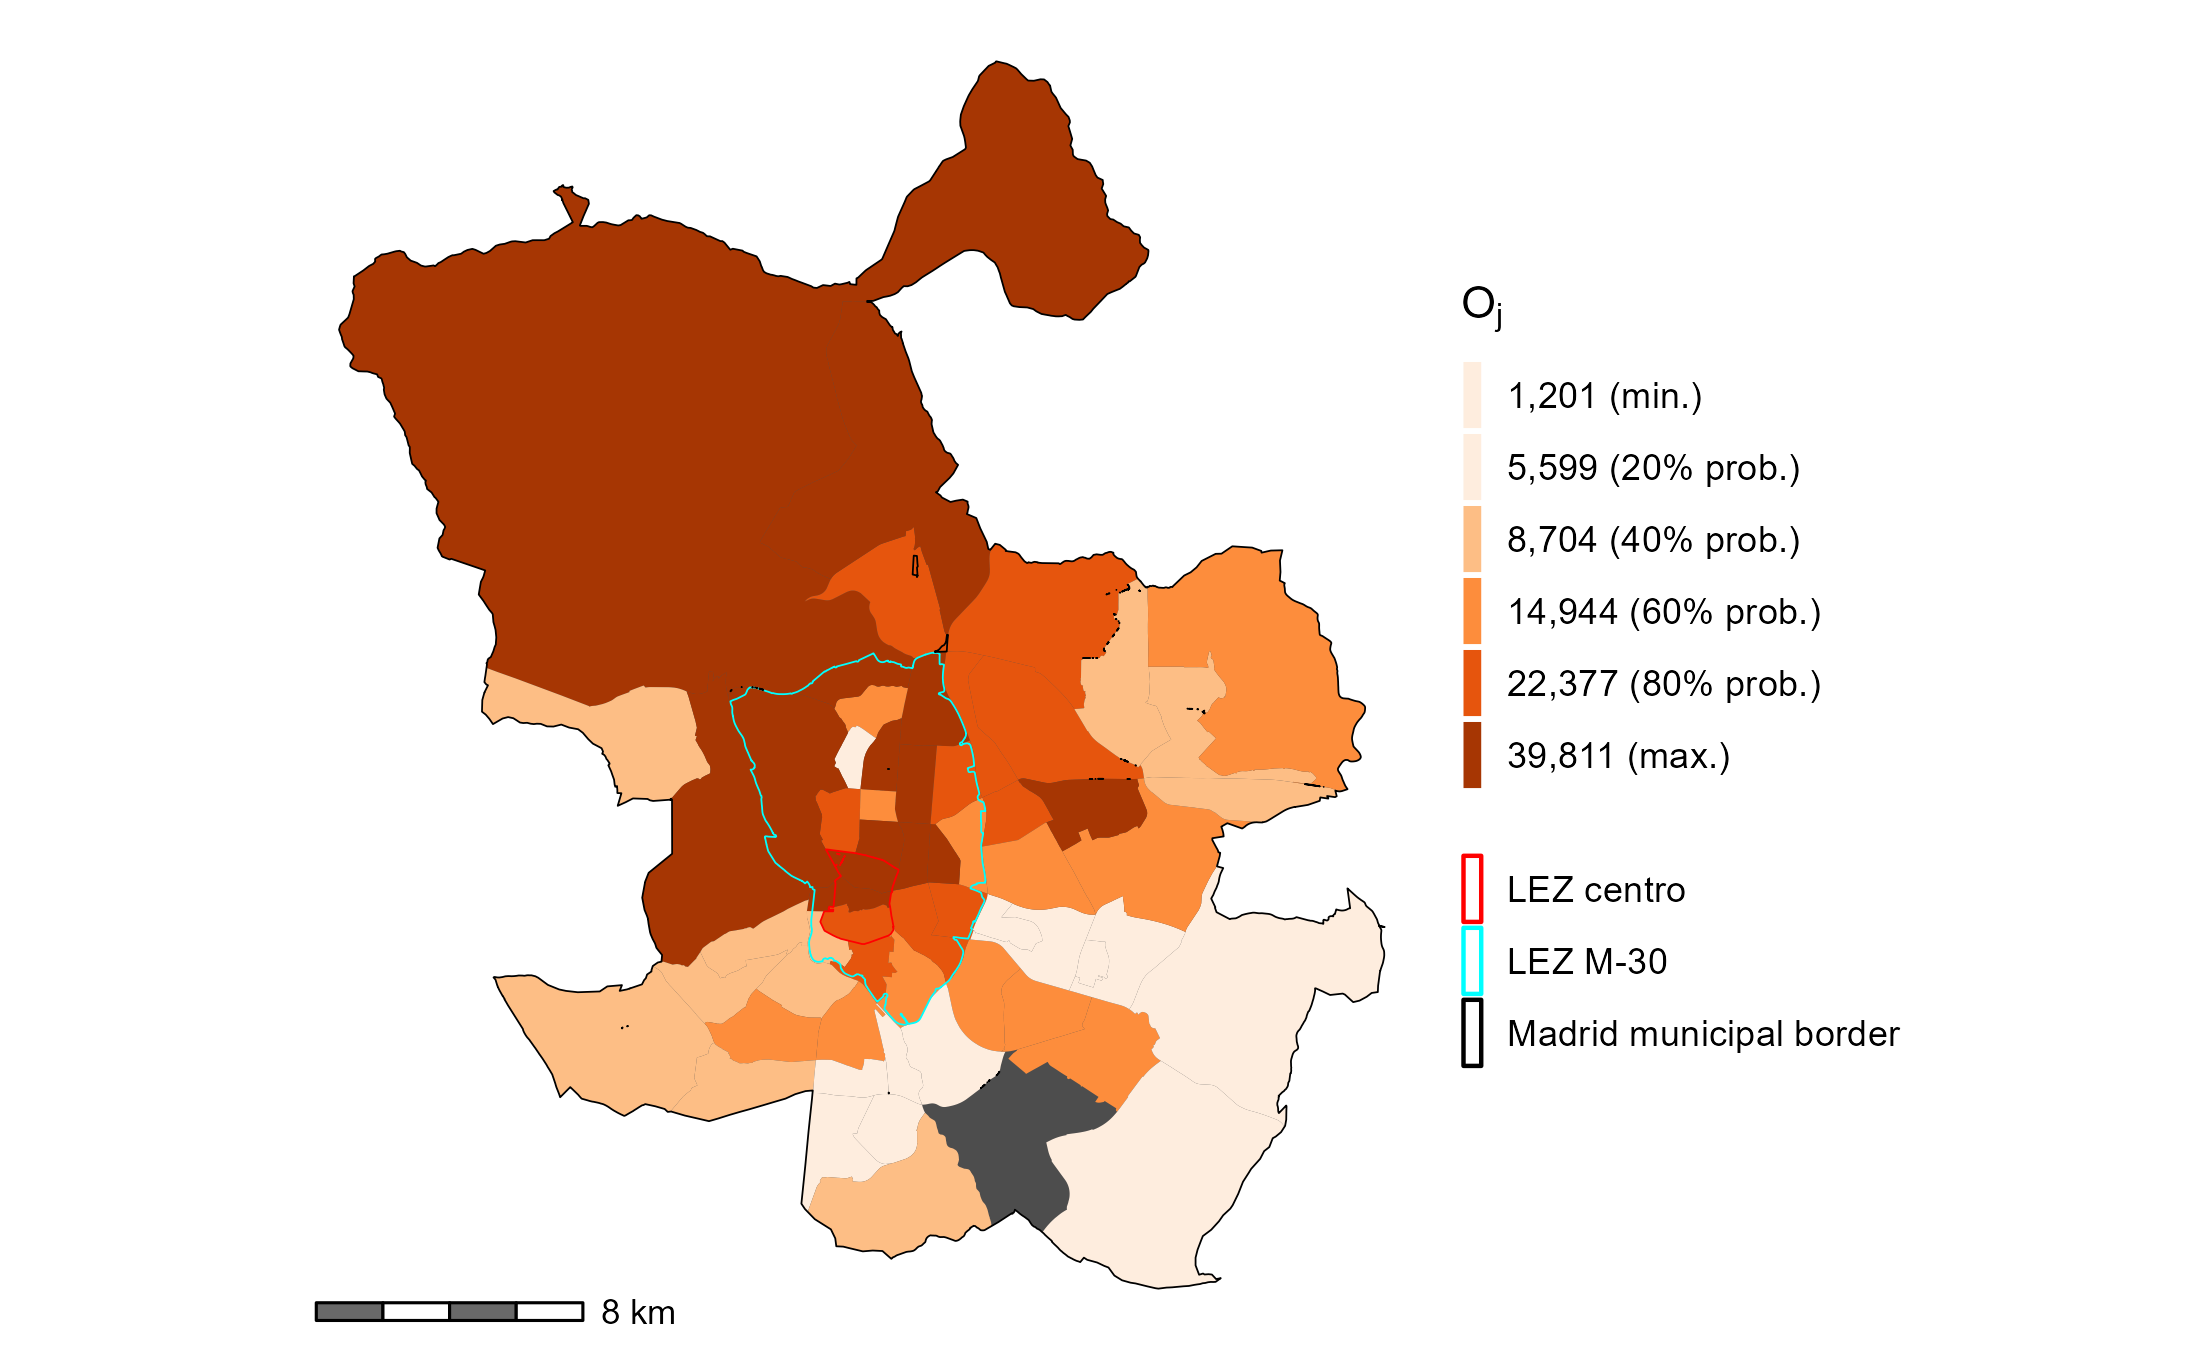
\includegraphics[width=1\linewidth]{images/i_jobs_zn208_plot} 

}

\caption{\label{fig:Fig2} Jobs $O_j$ taken by people living and working in Madrid as reported by the 2018 travel survey.}\label{fig:jobs-plot}
\end{figure}

\begin{figure}

{\centering 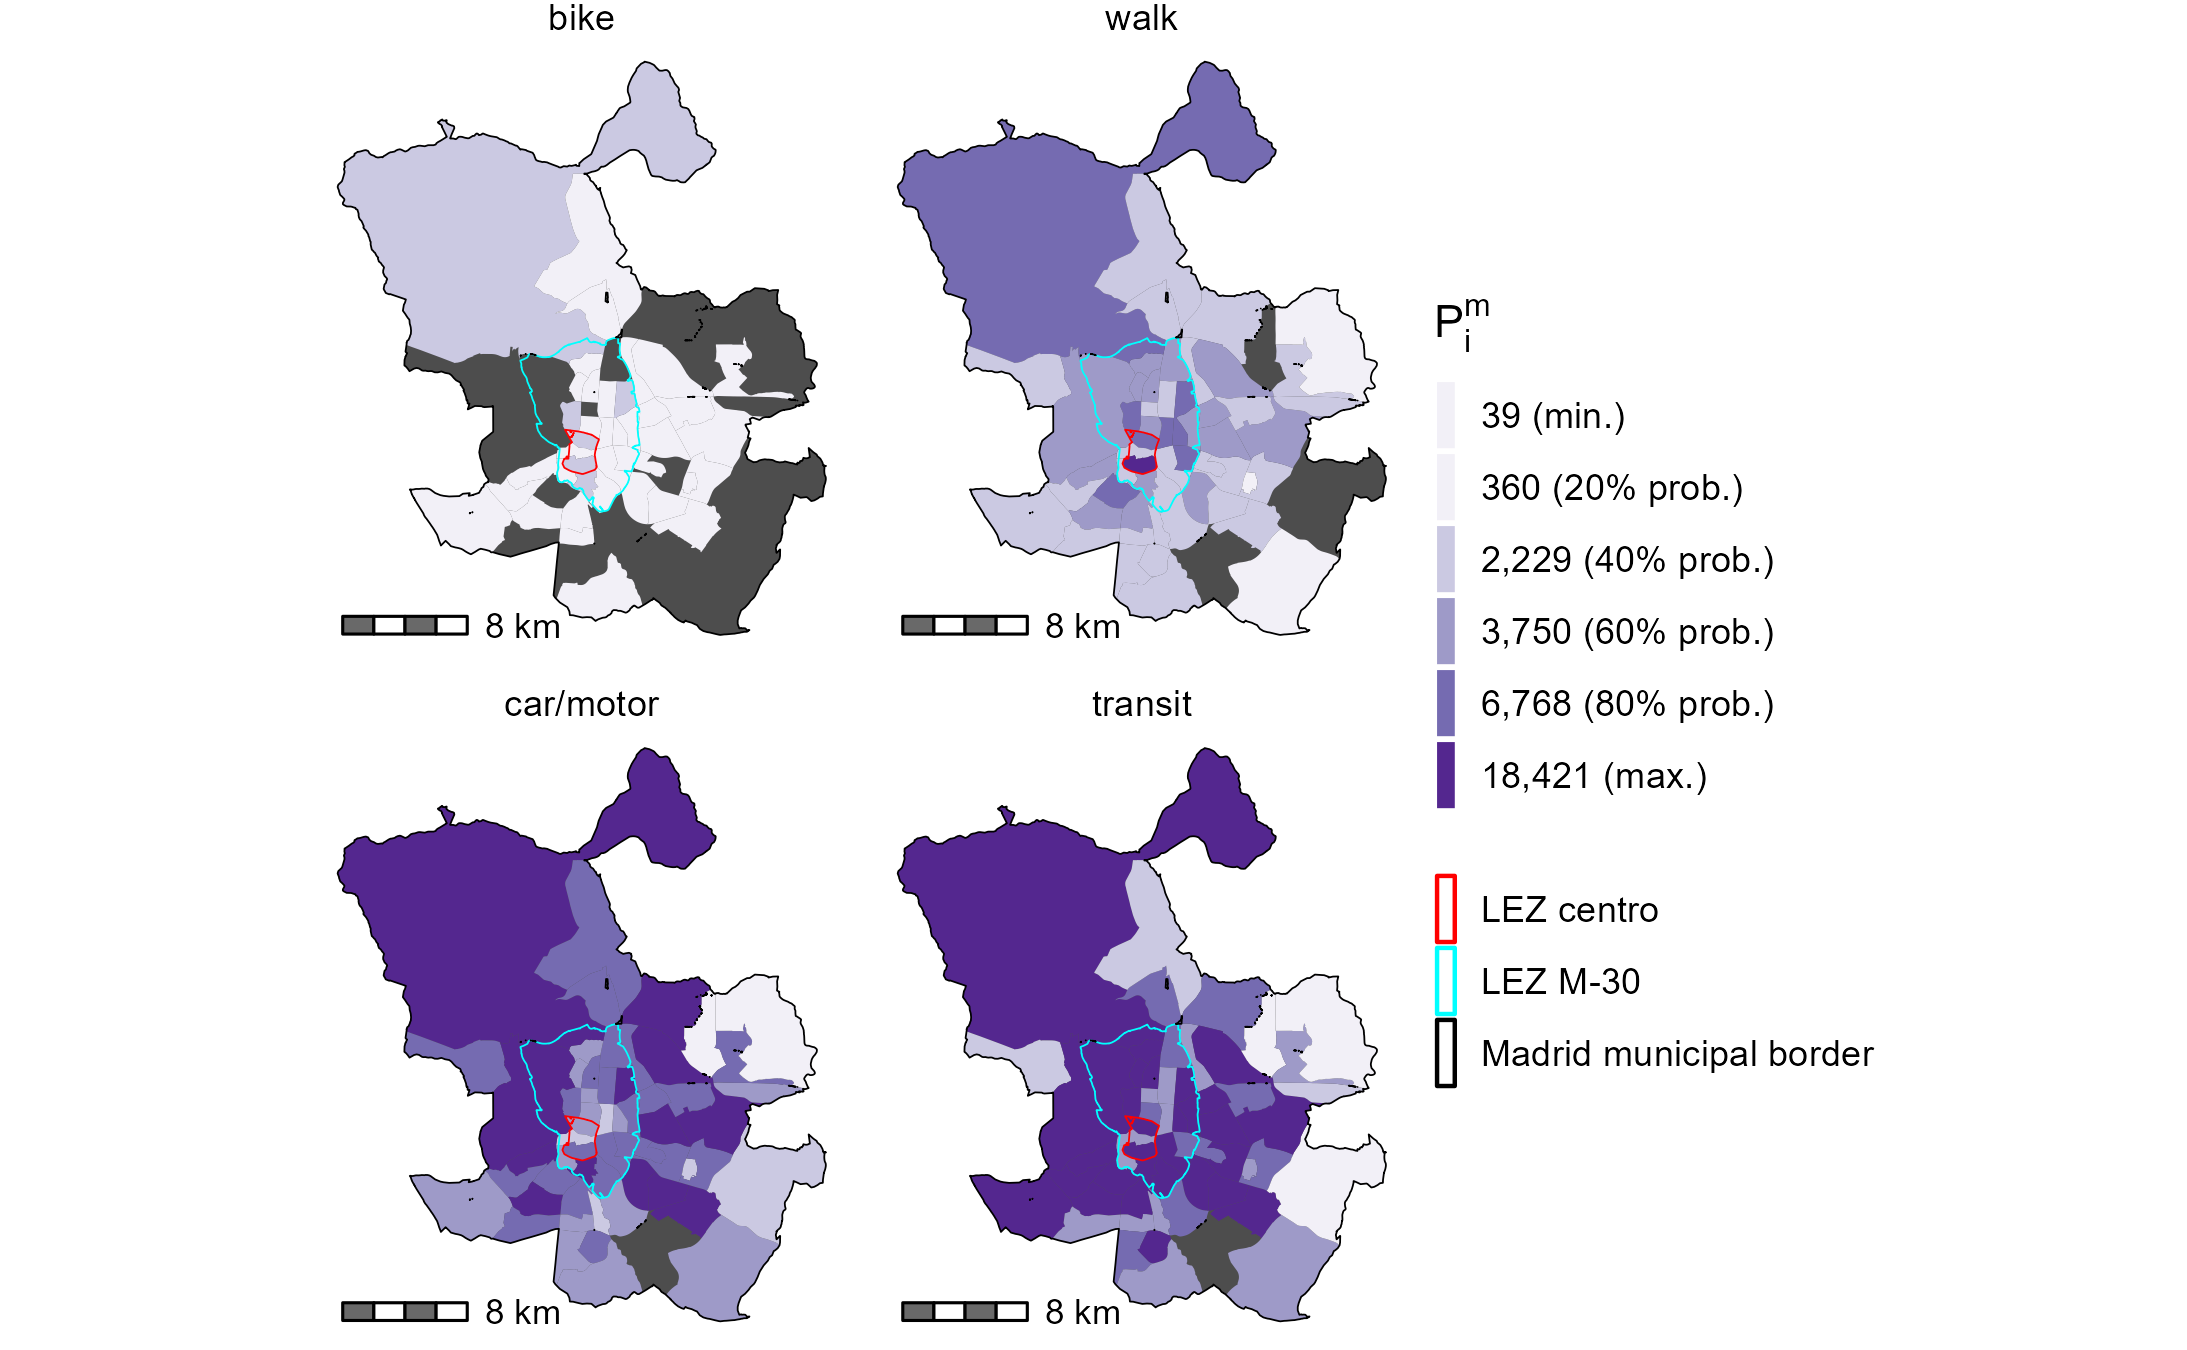
\includegraphics[width=1\linewidth]{images/im_populations_zn208_plot} 

}

\caption{\label{fig:Fig3} Population living and working in Madrid, by four summarized modal categories, $P^m_i$ as reported by the 2018 travel survey.}\label{fig:pop-plot}
\end{figure}

The 2018 Community of Madrid travel survey is the source of data for the
empirical example: it is a representative survey that reflects a
snap-shot of the travel patterns for one typical day of the working week
(e.g., n=222,744 trips with representative population elevation
factors). In this paper, a sample of the travel survey is used, namely
the residential home origin to work destination trips of all modes and
those that originate and end in Madrid. These totals are displayed in
Figure \ref{fig:Fig2} and Figure \ref{fig:Fig3}. Both figures are
displayed at the level of traffic analysis zones (\(i\) and \(j\)) that
correspond to the 2018 travel survey. The red boundary represents the
LEZ Centro in effect in 2017 and thus those travel patterns of
car-restriction reflected in the 2018 travel survey data. The cyan
boundary represents the LEZ that will be within the boundaries of the
M-30 highway in 2023 and is present in the plots as a spatial reference
for areas in proximity to the LEZ Centro.

The total sum of jobs \(O_j\) that are held are shown in Figure
\ref{fig:Fig2} and the populations that go to a work destination by four
modal categories \(P^m_i\), is reflected in Figure \ref{fig:Fig3}. The
modal categories represented in Figure \ref{fig:Fig3} were summarized
for the following trip mode types: - Car/motor: all cars and operating
modes (e.g., cab, private driver, company, rental care, main driver,
passenger, etc.) and all public, private or company motorcycle/mopeds. -
Transit: all bus, trams, and trains - Bike: all bicycle trips (e.g.,
private, public, or company bike trips) and ``other'' types of
micromobility options - Walk: walking or by foot

From Figure \ref{fig:Fig2}, it can be seen that the largest
concentration of jobs are within, near, and to the north of the LEZ
Centro.. The population that is accessing those jobs by mode (Figure
\ref{fig:Fig3}), appear spatially distinct. Car and transit trips
represent 37\% and 47\% of the modal share respectively. The population
that travels using transit is more spatially distributed than those
using cars - particularly near and within LEZ Centro. This distribution
could be a result of a variety of factors including: transit coverage
and service within with city, effective car infrastructure outside of
the M-30, and/or the impact of the Central LEZ itself.

From Figure \ref{fig:Fig2}, it can also be seen that biking and walking
trips are less common than motorized trips at 1\% and 15\% respectively.
The distribution of walking and biking trips appear to be similar to
that of transit trips. This is to be expected as active transport and a
higher diversity of land-use spatially occurs with transit
infrastructure.

The travel time for each trip is provided within the 2018 survey. These
travel times, per modal category, are used to calibrate mode specific
travel impedance functions \(f^m(c_{ij}^m)\). To illustrate the modal
differences in travel lengths, summary descriptive per mode are detailed
as follows:

\begin{itemize}
\tightlist
\item
  Car/motor: 36 min (Min:0min, Q2: 15 min, Q3: 55 min, Max: 120 min)
\item
  Transit: 55 min (Min:1 min, Q2: 30 min, Q3: 80 min, Max: 120 min)
\item
  Bike: 34 min (Min:5 min, Q2: 15 min, Q3: 40 min, Max: 115 min)
\item
  Walk: 27 min (Min:1 min, Q2: 10 min, Q3: 45 min, Max: 119 min)
\end{itemize}

To calculate the mode specific travel impedance functions
\(f^m(c_{ij}^m)\) from the travel times, a concept known as the trip
length distribution (TLD) is used. A TLD represents the proportion of
trips that are taken at a specific travel cost such as travel time. This
distribution is then used to derive impedance functions as done in
previous accessibility research \citep[e.g., works
of][\citet{horbachov_theoretical_2018}, and
\citet{batista_estimation_2019}]{lopez_2017_spatial}. Maximum likelihood
estimation and the Nelder-Mead method for direct optimization available
within the R \{fitdistrplus\} package \citep{fitdistrplus_2015} is used.
As shown as shown in Figure \ref{fig:Fig4}, based on goodness-of-fit
criteria and associated diagnostics, the gamma and log-normal
probability density function (line curves) are selected as best fitting
curves for the motorized and non-motorized modes respectively. The
selection of functional form aligns with examples used in the literature
(e.g., \citet{reggianiAccessibilityImpedanceForms2011}). Overall, the
plots in Figure \ref{fig:Fig4} display the probability of travel given a
trip travel time, based on actual travel behaviour from the 2018 survey.
These `probability of travel' at each travel time for each mode are
realized observations reflect the land-use, the transport system, and
the population travel preferences/behaviour in Madrid.

\begin{figure}

{\centering 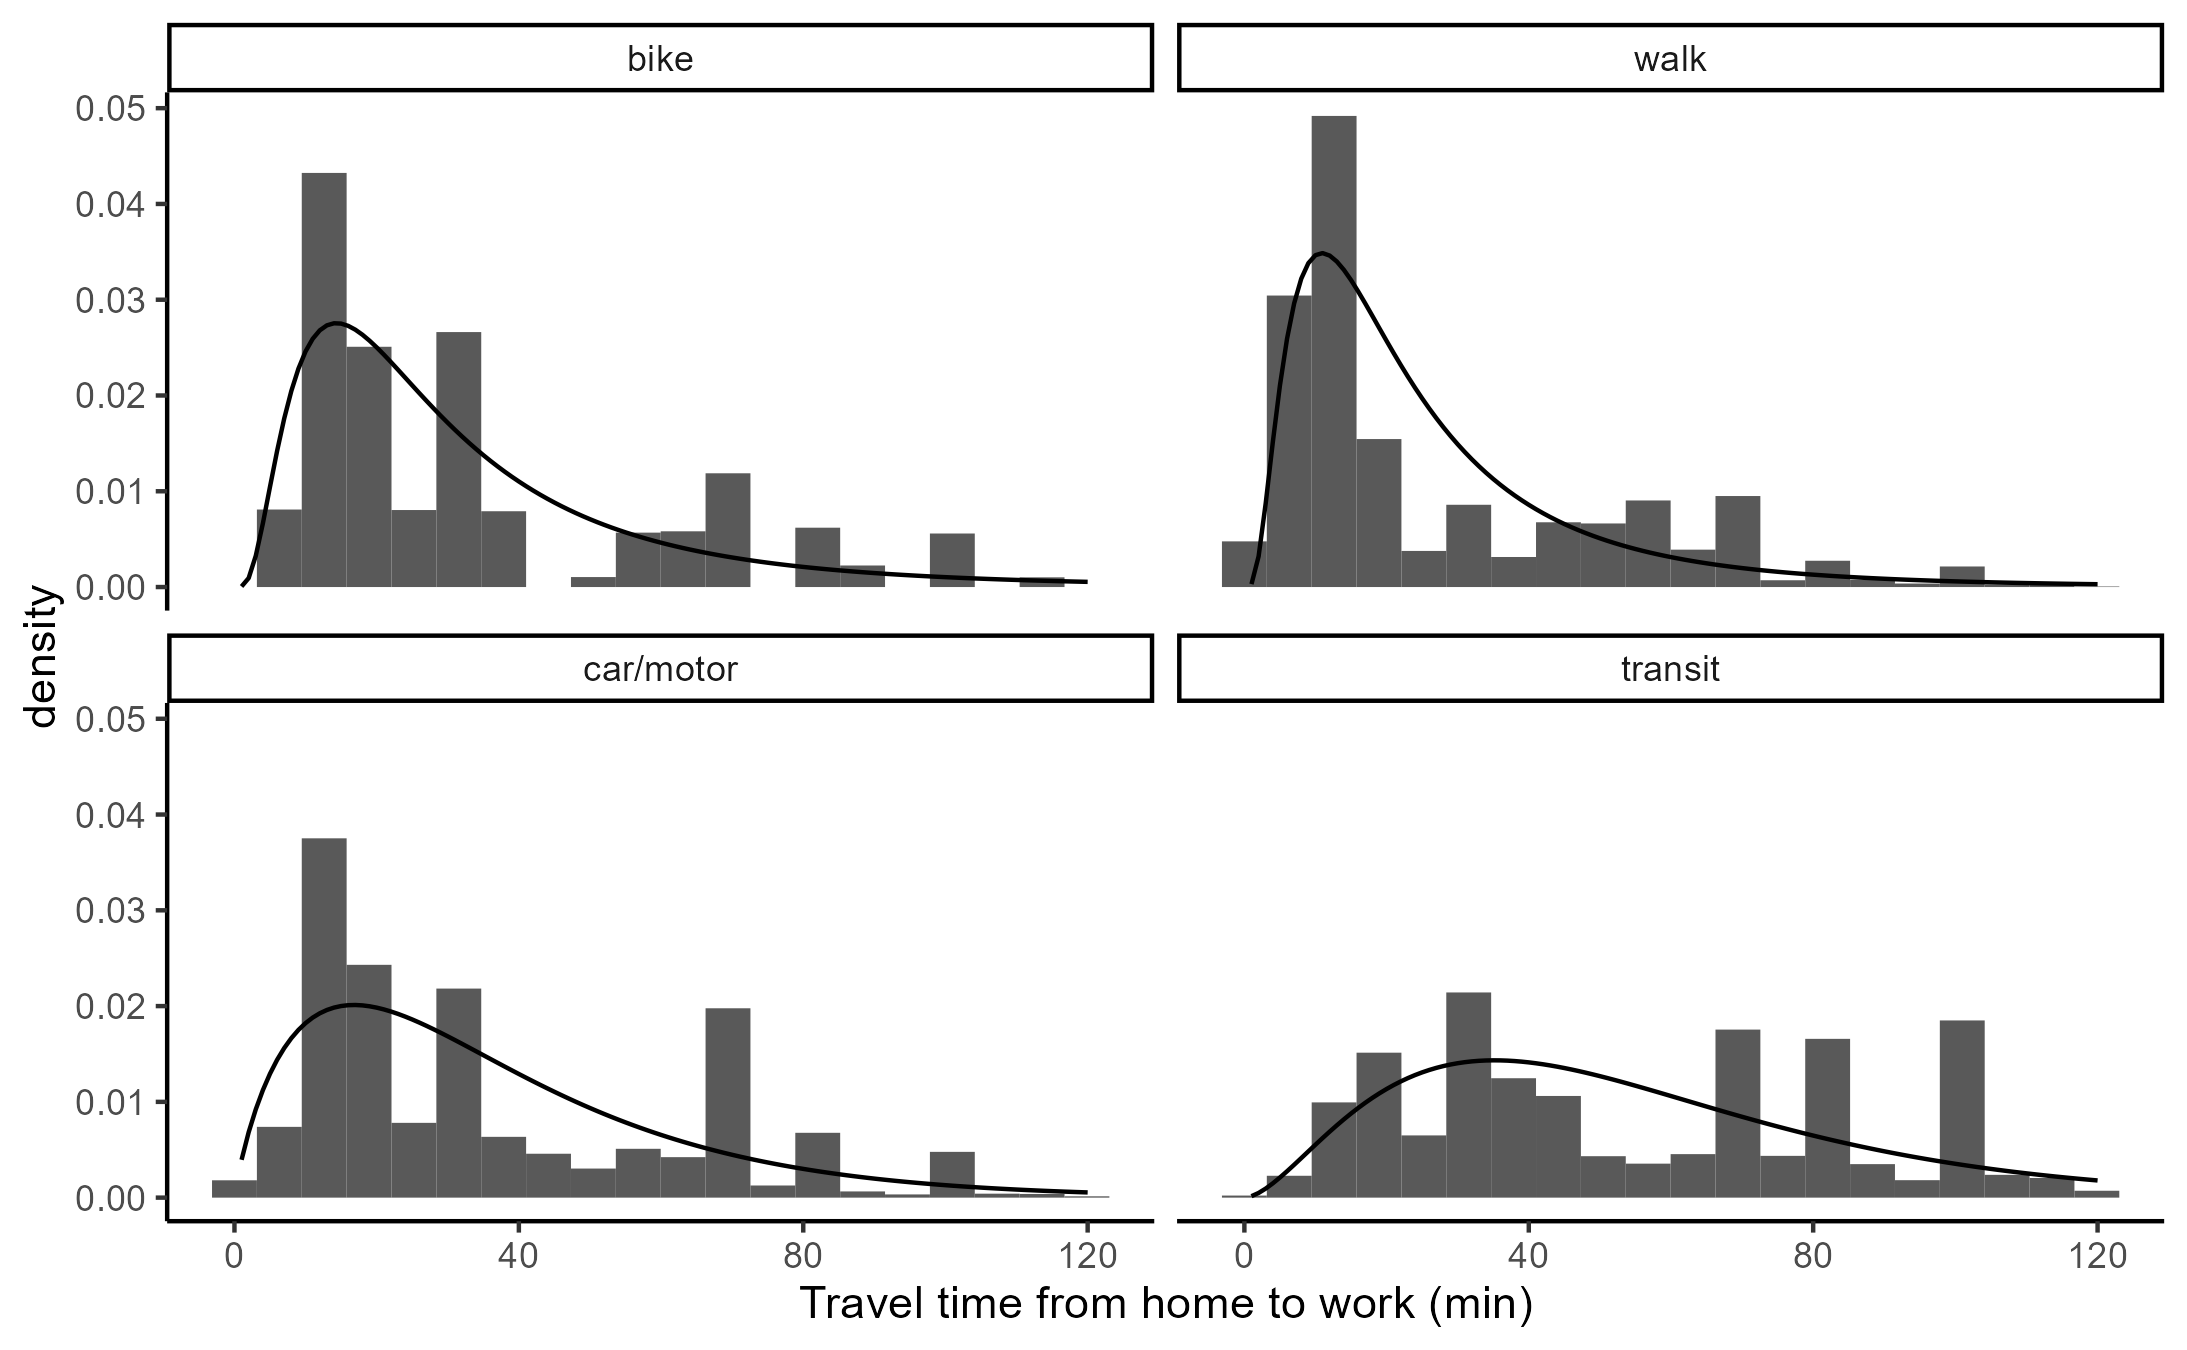
\includegraphics[width=1\linewidth]{images/tlds_curves_m_plot} 

}

\caption{\label{fig:Fig4} Fitted impedance function curve (line) against empirical TLD (bars) per mode.}\label{fig:tlds-curves-m-plot}
\end{figure}

\hypertarget{results-spatial-availability-v_im-and-v_i}{%
\subsection{\texorpdfstring{Results: spatial availability \(V_i^m\) and
\(V_i\)}{Results: spatial availability V\_i\^{}m and V\_i}}\label{results-spatial-availability-v_im-and-v_i}}

Using the data inputs outlined, spatial availability of jobs are
calculated for each of the four modal categories at the level of traffic
analysis zones in Madrid, \(V_i^m\). The spatial distribution of the
resulting calculations are demonstrated in this section.

\begin{figure}

{\centering 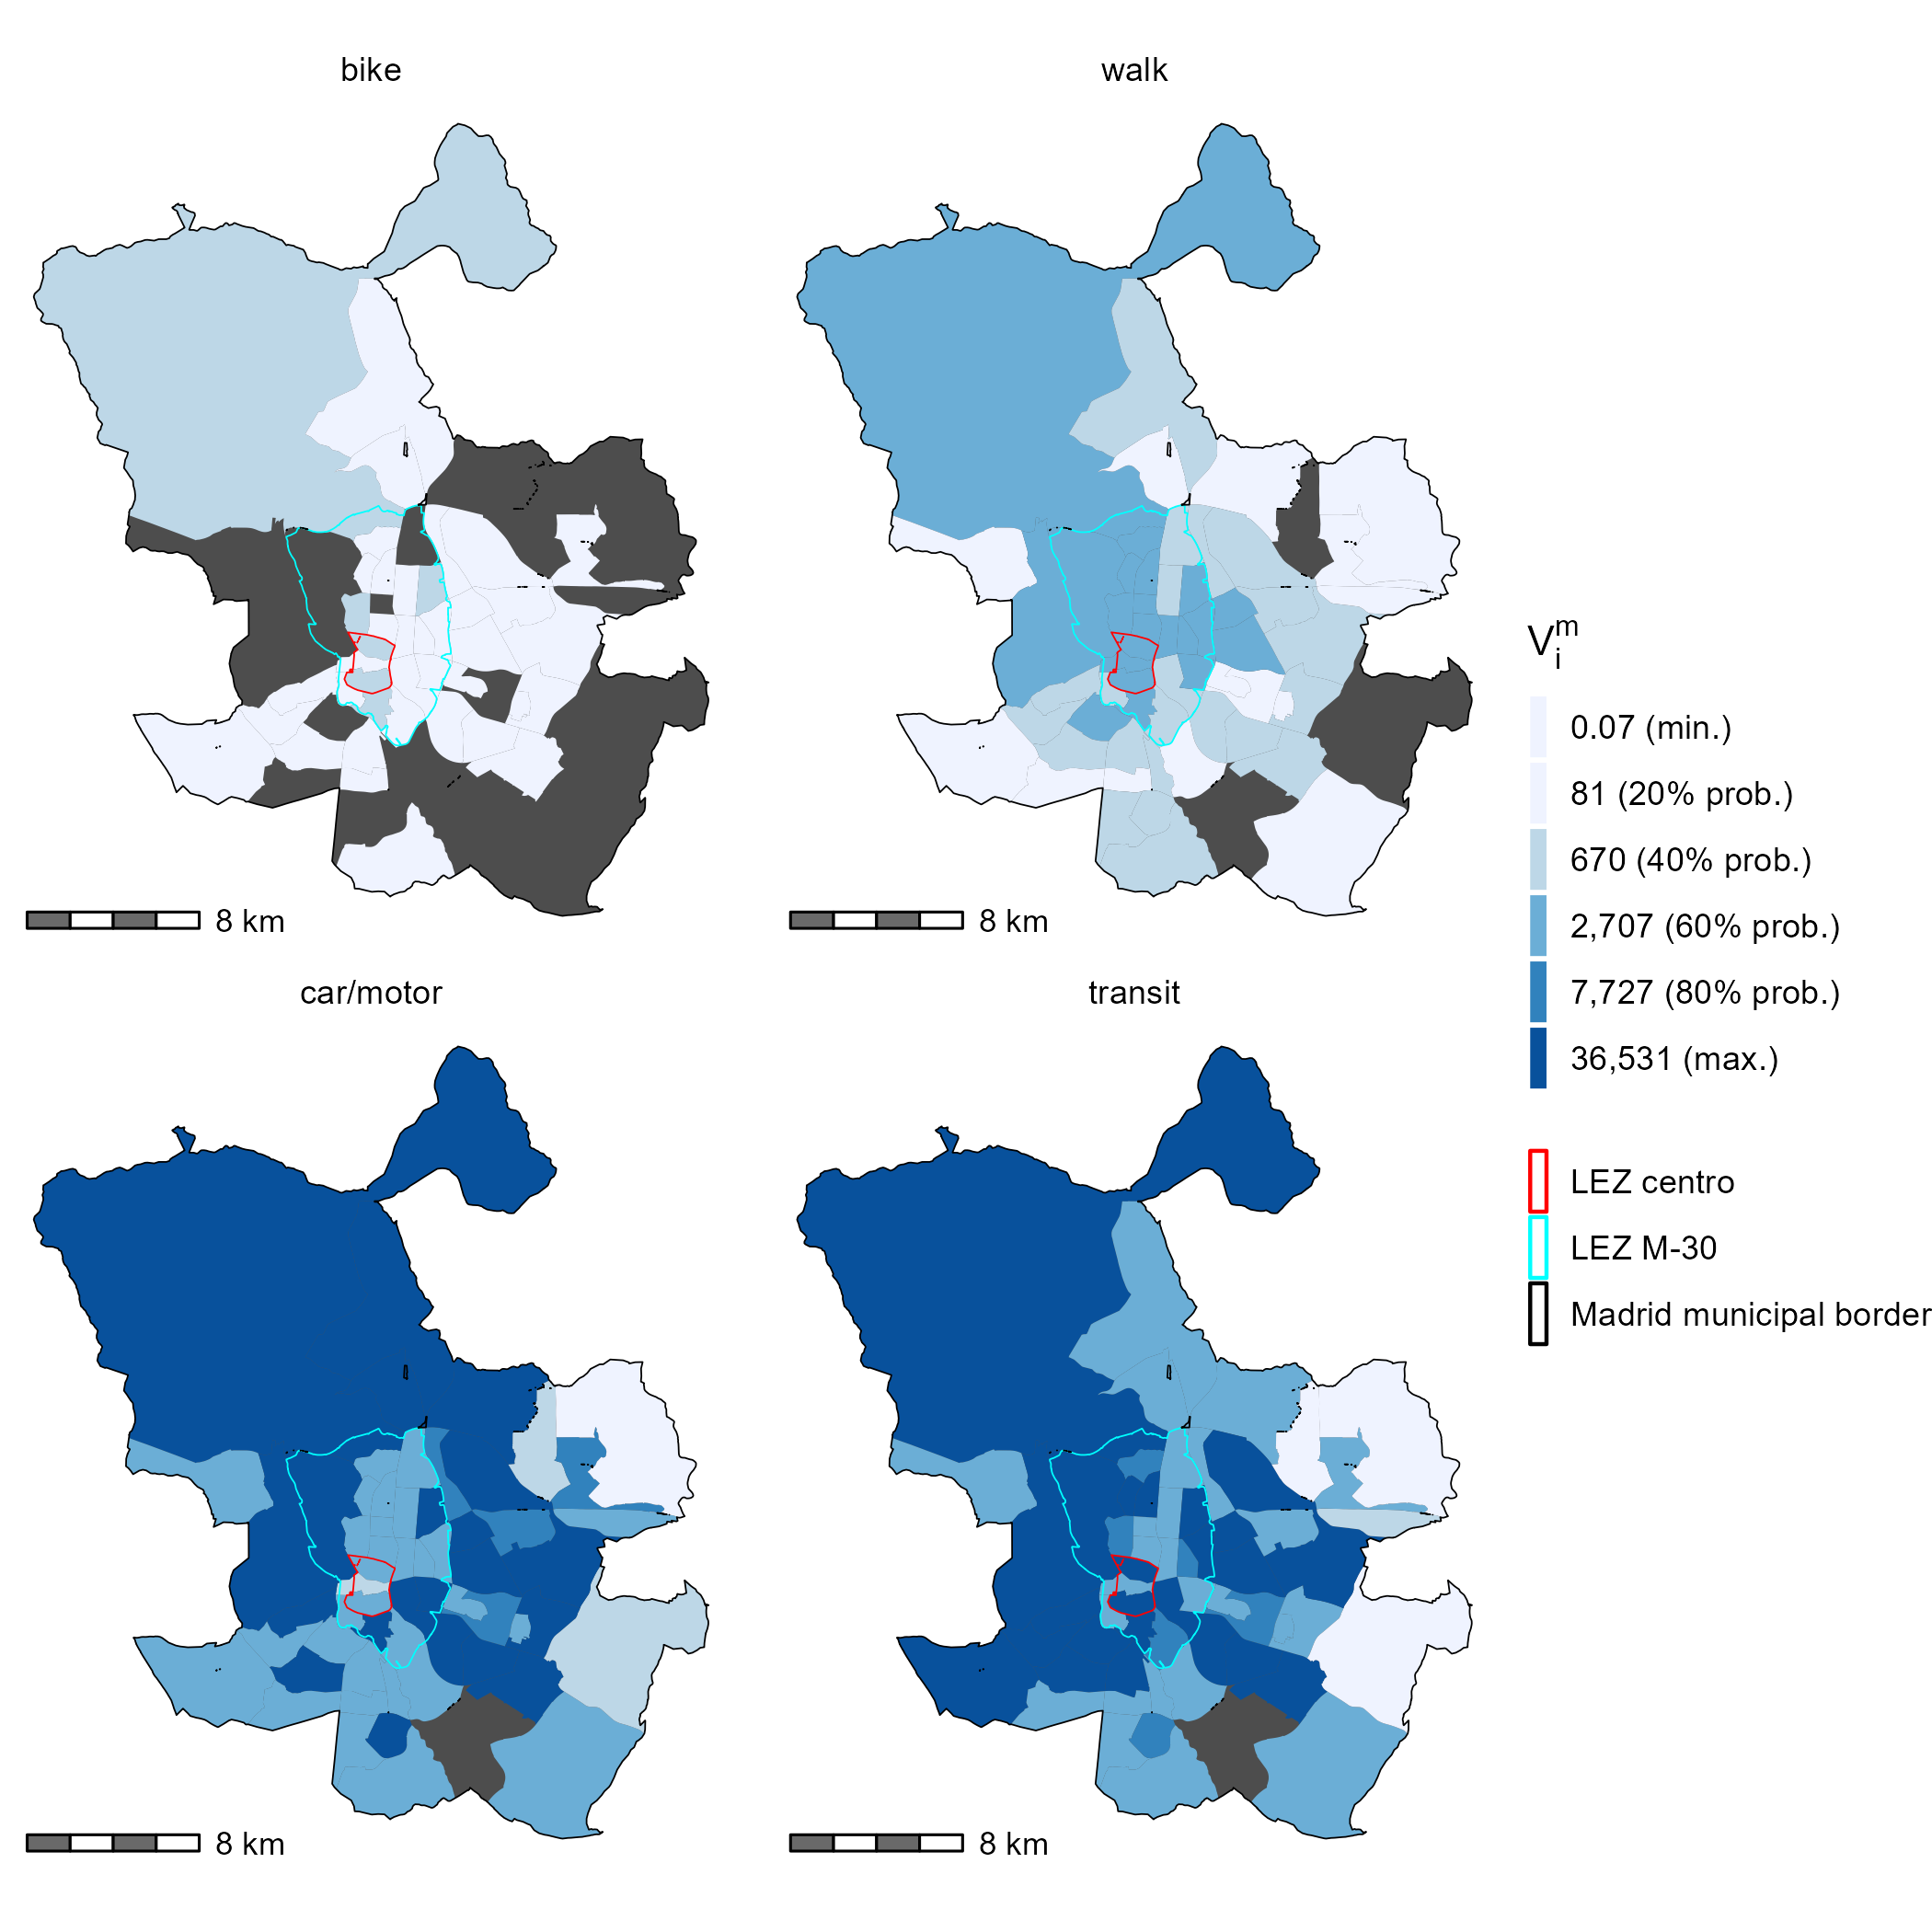
\includegraphics[width=1\linewidth]{images/SA_im_V_zn208_plot} 

}

\caption{\label{fig:Fig5} Spatial availability of job opportunities per origin and mode $V_i^m$ in Madrid as reported by the home-to-work origin destination flows from the 2018 travel survey. 2017 central LEZ is shown in blue. 2023 expanded LEZ boundaries shown in red.}\label{fig:SA-m-plot}
\end{figure}

Figure \ref{fig:Fig5} displays the spatial availability values for the
four modal categories at the level of the spatial units used in the 2018
travel survey. These values represent a proportion of the total number
of the 847,574 jobs in the region that are \emph{spatially available} to
the population located at the \(i\) based on the travel impedance of the
mode (relative to the travel impedance of all modes) and the mode-using
population size at the \(i\) (relative to the population size of all
modes and \(i\)). Since population, their job locations, and associated
travel times are used to calculate \(V_i^m\), Figure \ref{fig:Fig5}
demonstrates values that represent the \emph{realized} spatial
availability of jobs in Madrid. In other words, if someone decided to
move into a neighbourhood at an \(i\), the amount of jobs that are
spatially available to them based on the population within their \(i\)
and their travel impedance for their used \(m\), both relative to the
city, is captured by the value of \(V_i^m\).

In Figure \ref{fig:Fig5}, the difference in the magnitudes of \(V_i^m\)
values between \(m\) can be observed. The majority of \(V_i^m\) is
allocated to the populations using motorized modes. This is to be
expected as commuting using motorized modes represents 84\% of the
population (37\% (car/motor) and 47\% (transit)). However, these modal
options capture 95\% of the total spatial availability in Madrid. In
particular, the car/motor using population is allocated
disproportionately more \(V_i^m\) than its modal population (37\% of the
population vs.~48\% of the \(V_i^m\)) compare to the transit using
population and its relatively proportional \(V_i^m\) value (15\% of the
population vs.~47\% \(V_i^m\)).

How does the \(V_i^m\) advantage allocated to car-using population
arise? From the perceptive of finite opportunities, \(V_i^m\) is
allocated to car-using populations from less competitive modal
populations. How competitive one mode is compared to other modes varies
spatially, but overall car-using populations capture more opportunities
per car-using population than other modal populations. Namely, though
walking and cycling populations represent 14.74\% and 1.16\%
respectively, \(V_i^m={walk}\) and \(V_i^m={bike}\) is 4.43\% and 0.23\%
in the region respectively. These modes are less competitive, especially
compared to the car/motor mode, as a result of: 1) their lower travel
impedance values at longer travel times (see Figure \ref{fig:Fig4} at
travel times beyond \textasciitilde30 minutes), 2) their low population
values values overall, and 3) higher populations present in origins with
high motorized mode commuting. These factors all contribute to the the
car/motor mode being most advantaged in capturing spatially available
job opportunities overall.

\begin{figure}

{\centering 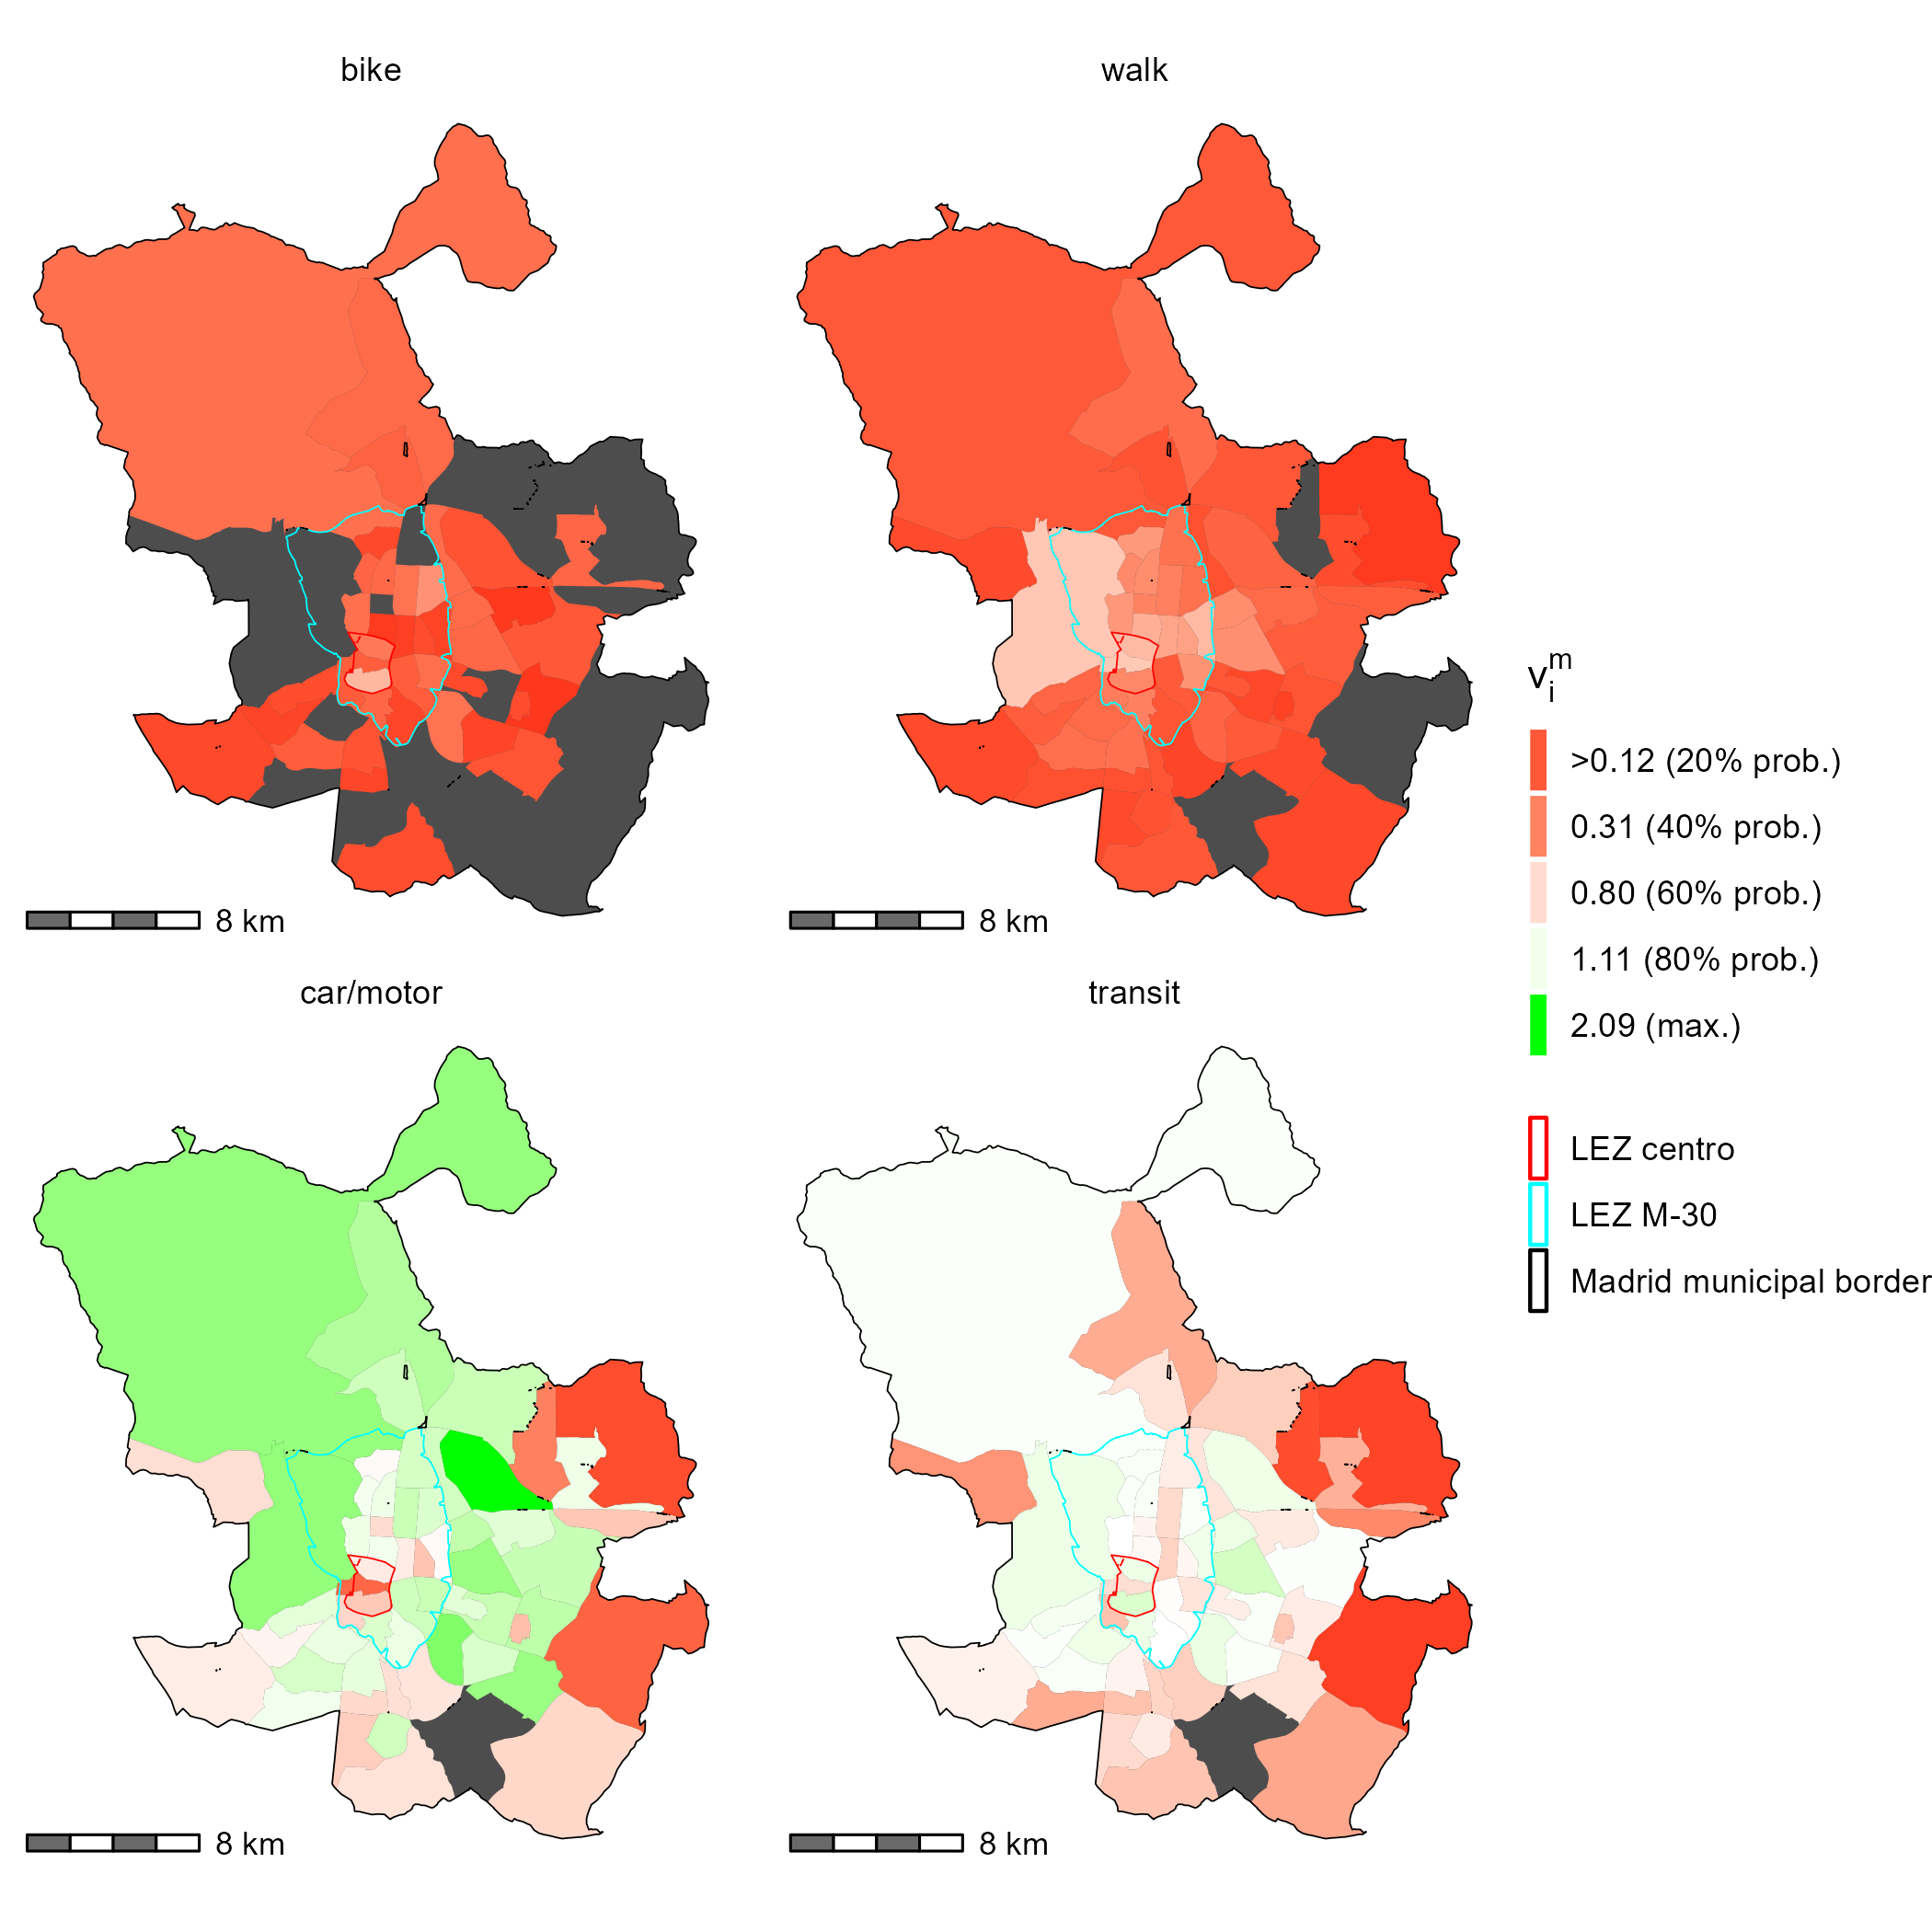
\includegraphics[width=1\linewidth]{images/SA_im_vv_zn208_plot} 

}

\caption{\label{fig:Fig6} Spatial availability of job opportunities per capita per origin and mode $v_i^m$ in Madrid as reported by the home-to-work origin destination flows from the 2018 travel survey. 2017 central LEZ is shown in blue. 2023 expanded LEZ boundaries shown in red.}\label{fig:SA-per-capita-m-plot}
\end{figure}

Furthermore, there are spatial differences in the competitive advantage
of spatial availability between modes. Figure \ref{fig:Fig6} visualizes
\(v_i^m\), the spatial availability divided by the mode population.
\(v_i^m\) values above 1 are represented in increasing red shades,
values below 1 are represented in increasingly green shades, and values
equal to 1 are white. These plots illustrates the discussion of the
disproportionately high over representation of spatial availability
relative to the mode-using population in many of the origins for the car
plot (bottom right, denoted with green \(v_i^m\) values above 1). These
plots also visualize areas that are awarded disproportionately low
spatial availability, represented in shades of red. Interestingly,
spatial availability for the car mode within the LEZ Centro is below 1
(red). For all other modes, the area with the LEZ is relatively higher
than the modal averages or even green in the case transit-using
populations. This difference in spatial availability can be seen as a
direct result of the LEZ Centro - the observed reduction of
opportunities within the LEZ Centro boundaries being accessed by
car-using populations allows lesser competitive modes to interact with
these opportunities.

\begin{figure}

{\centering 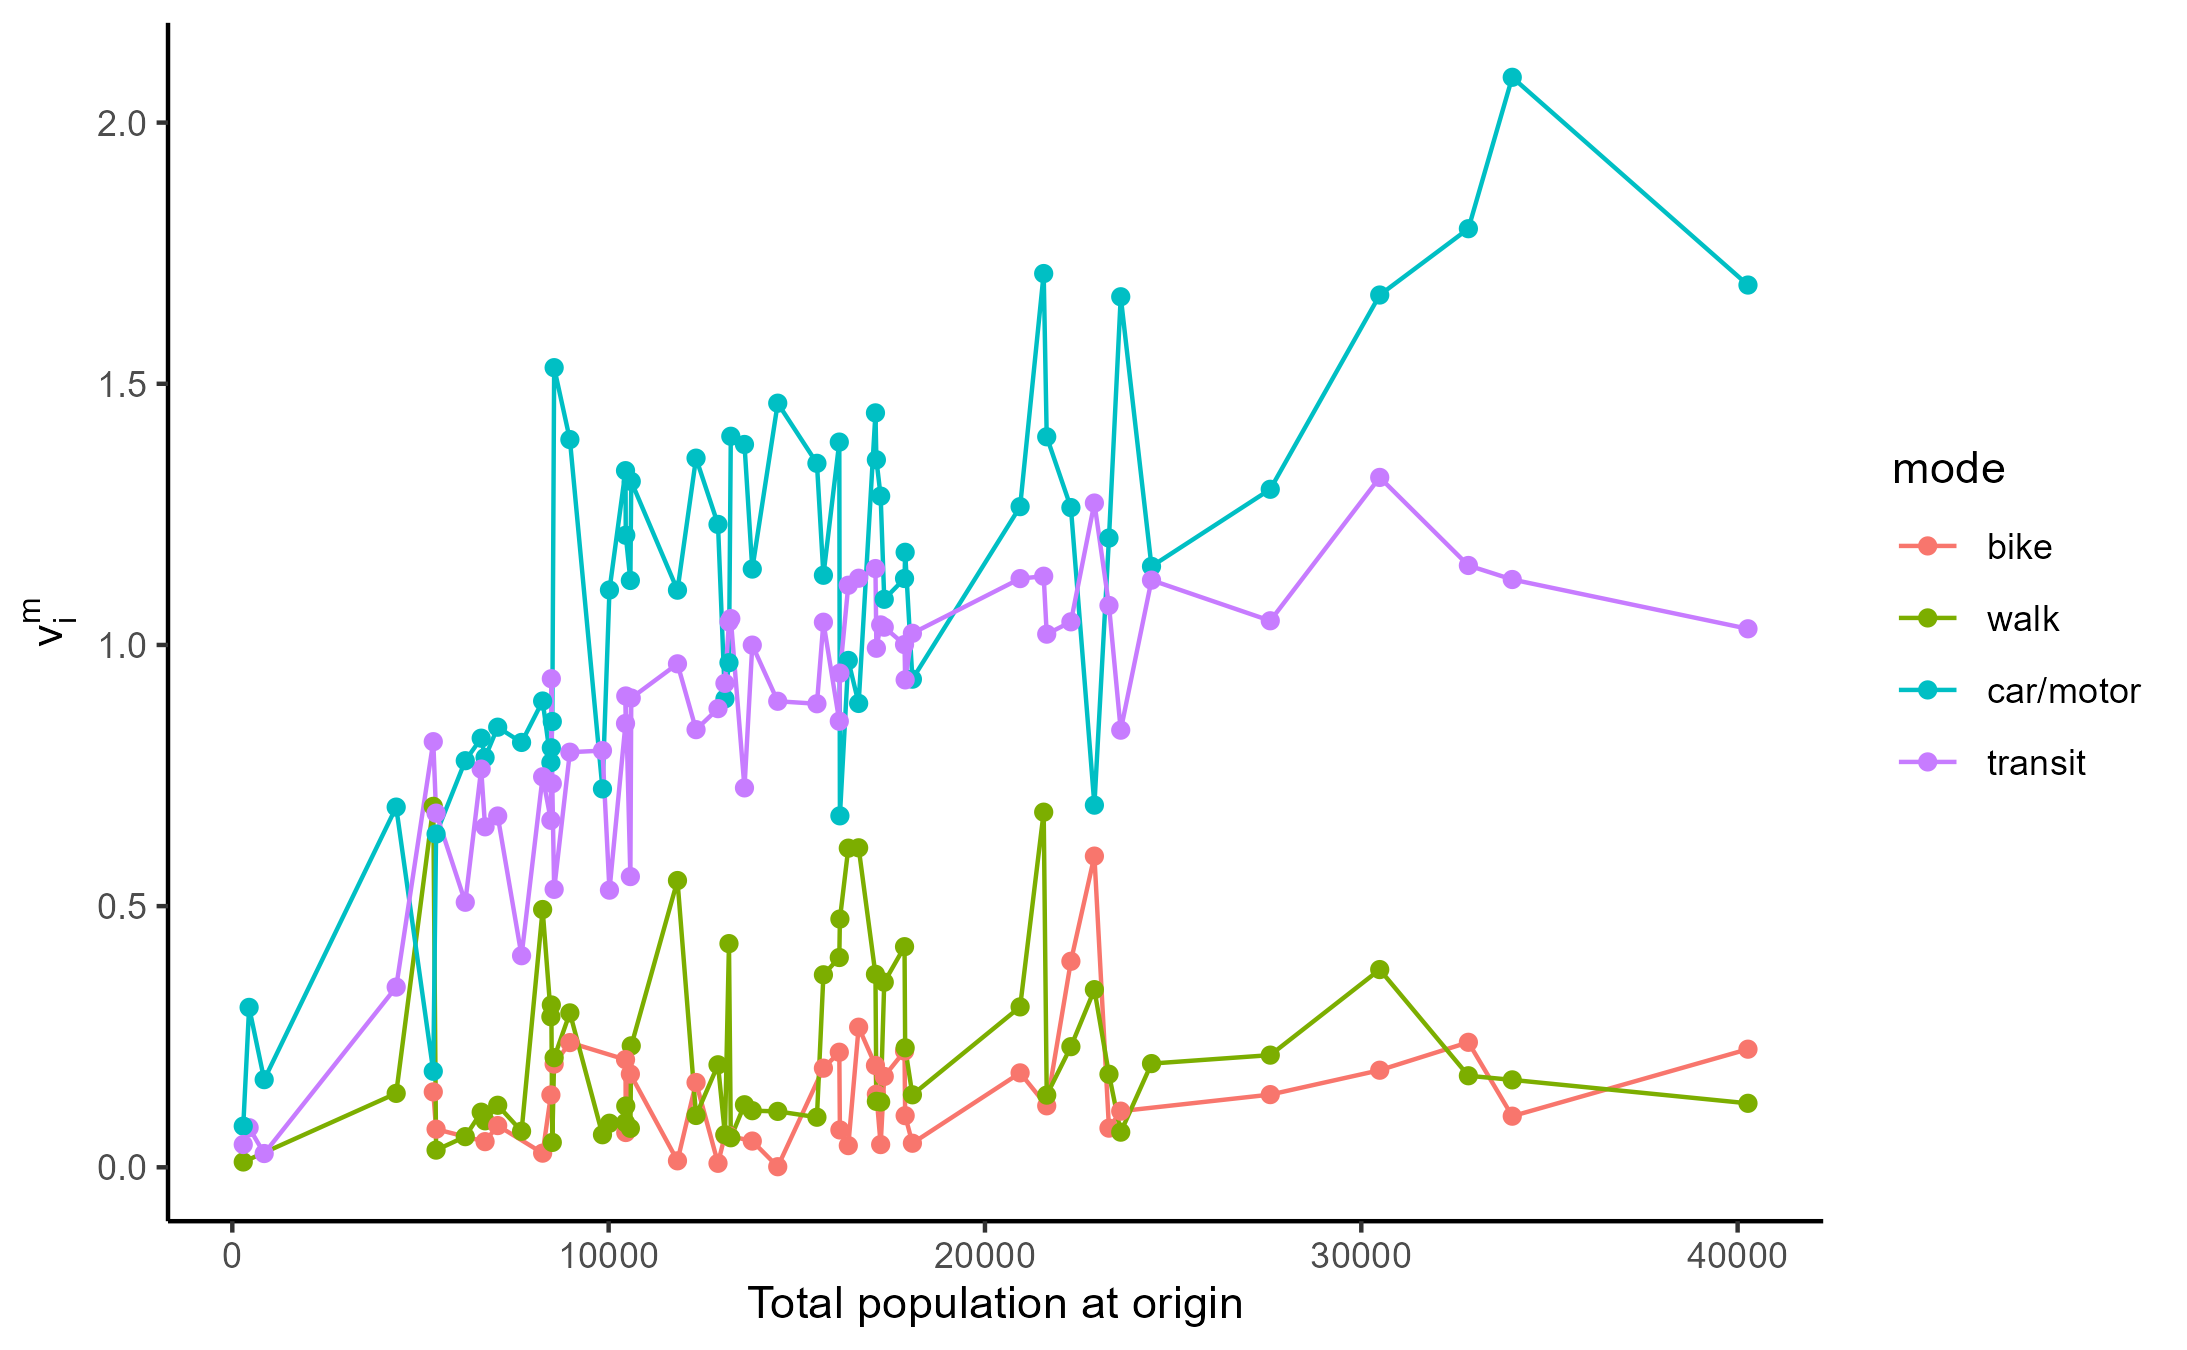
\includegraphics[width=1\linewidth]{images/v_im_per_pop_plot} 

}

\caption{\label{fig:Fig7} Spatial availability of job opportunities per capita per origin and mode $v_i^m$ in Madrid as reported by the home-to-work origin destination flows from the 2018 travel survey represented by sorted total population per origin.}\label{fig:SA-per-capita-m-linear-plot}
\end{figure}

Furthermore, Figure \ref{fig:Fig6} makes it evident that transit-using
population's spatial availability to jobs is relatively balanced (i.e.,
many zones are white). Additionally, values for non-motorized modes are
higher in origins that have higher transit accessibility. Transit
accessibility and non-motorized modes do not appear to be in direct
competition as a result of different travel impedance weighting . It is
not visually clear in the plots but as demonstrated in a line plot of
\(v_i^m\) sorted by total population in Figure \ref{fig:Fig7}, it can be
observed that transit is only close to or above 1 when car accessibility
is relatively low. From Figure \ref{fig:Fig7} we can also observe that
overall, motorized modes capture more spatial availability per capita
than non-motorized modes.

\hypertarget{discussion-and-conclusions}{%
\subsection{Discussion and
conclusions}\label{discussion-and-conclusions}}

Location-based accessibility measures like the Hansen-type measure,
Shen-type measure, and spatial availability all have a commonality -
they are a weighted sum of opportunities assigned to each spatial unit
in a region. In this way, they can be interpreted as a score that
represents how many opportunities can be potentially interacted with by
the population at each spatial unit. How the weight and sum of the
potentially interacted opportunities is what defines the type of
accessibility measure. Within this paper, the location-based
accessibility measures known as spatial availability, a singly-
\emph{constrained} and \emph{competitive} measure, is extended for the
case of capturing multimodal accessibility to opportunities. A synthetic
example and then an empirical case of LEZ in Madrid are detailed to
demonstrate the multimodal extension of the spatial availability
measure.

The spatial availability measure is capable of capturing a new
interpretation of multimodal competition that previous accessibility
measures have not yet done. We can hypothesis that populations using
modes with lower travel impedance, when competing for a finite set of
opportunities, will capture more opportunities. However, with spatial
availability, the number of spatially available opportunities that are
captured (of the total opportunities in the region) by each mode can be
individually calculated. From there, the difference between how many
spatially available opportunities one mode captures versus another can
be investigated.

The flexibility and need for an accessibility measure such as spatial
availability is pertinent in policy scenario evaluation. As showcased in
the empirical example of the LEZ in Madrid, competition for job
opportunity availability highly varies spatially and between modes. The
car and transit modes have the highest spatial availability, with the
car mode having highest availability with exception to the areas with
LEZ Centro. This finding reflects real conditions: since car travel has
been highly restricted within the LEZ Centro, much fewer car-using
population and much more people are entering using other modes relative
to the areas surrounding the LEZ Centro. This difference in car-using
population within and immediately outside the LEZ Centro increases the
competitiveness of the transit-using population (the second most
competitive mode) as well as the non-motorized modes.

Currently, conventional \emph{non-constrained} accessibility measures
are difficult for planners to operationalize for a variety of reasons.
They have also been criticized for being difficult to compute and
difficult to interpret as they are a ratio of supply to demand
\citep{levinsonTransportAccessManual2020}. With spatial availability,
the magnitude of opportunities that are available as a proportion of all
the opportunities in the region is equal to \(V_i\). As a result of its
proportional allocation mechanism it can be easily extended into
multimodal applications, pertinent to model policy scenerios in our
cities that are becoming increasingly multimodal. This flexibility and
interpretation of the spatial availability measure allows for
manipulation of \(V_i^m\) values to investigate differences of
availability between neighbourhoods, modes, and regions, generate per
capita benchmarks, and/or generate average values per population-group.

From a spatial equity perspective, spatial availability measure can
provide researchers, policy makers, and citizens a newfound
interpretation of accessibility measures. With a plot of spatial
availability values, one can begin asking, how much is enough and what
level is too much. These interpretations were difficult to be made with
accessibility measures in the past.

\hypertarget{acknowledgements}{%
\subsection{Acknowledgements}\label{acknowledgements}}

This research was funded by the Canada Graduate Scholarship - Doctoral
Program (CGS D) by the Social Sciences and Humanities Research Council
(SSHRC).

\#AUTHOR CONTRIBUTIONS

The authors confirm contribution to the paper as follows: study
conception and design: AS, JSL, AP.; data collection: AS, JSL, AP.;
analysis and interpretation of results: AS, JSL, AP.; draft manuscript
preparation: AS, JSL, AP. All authors reviewed the results and approved
the final version of the manuscript.

--\textgreater{}

--\textgreater{}

\newpage
\bibliography{mybibfile.bib}


\end{document}
